\documentclass{report}
\usepackage{amsmath}
\usepackage{txfonts}
\usepackage{amsfonts}
\usepackage{amssymb}
\usepackage{mathtools}
\usepackage{geometry}
\usepackage{color}
\usepackage{parskip}
\setlength{\parskip}{1em}
\usepackage{tikz}
\usetikzlibrary{fadings}
\usetikzlibrary{patterns}
\usetikzlibrary{shadows.blur}
\usetikzlibrary{shapes}
\usepackage{multirow}
\newcommand\parrow[3][3ex]{%
 \begin{array}[t]{@{}c@{}} #2 \\
  \left\uparrow\vcenter{\hrule height #1}\right.\kern-\nulldelimiterspace\\
  \makebox[0pt]{\small#3}
  \end{array}%
}
\newcommand\parrowlong[3][6ex]{%
 \begin{array}[t]{@{}c@{}} #2 \\
  \left\uparrow\vcenter{\hrule height #1}\right.\kern-\nulldelimiterspace\\
  \makebox[0pt]{\small#3}
  \end{array}%
}

\geometry{a4paper, margin=1in}

\begin{document}

\setcounter{chapter}{1}

\chapter{Boundary Value Problems}

\section{BVP 1(A): Diffusion of Heat in a Thin Bar, Ends Maintained at $0^\circ$}

Thin rod of length $L$, ends maintained at $0^\circ$, initial temperature $f(x)$, no heat generation, or absorption.\\

\begin{center}
    \begin{tabular}{cc}
    \tikzset{every picture/.style={line width=0.75pt}} 
    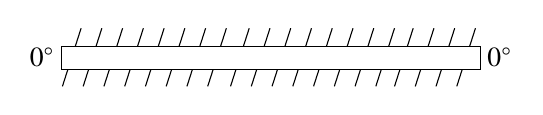
\begin{tikzpicture}[x=0.75pt,y=0.75pt,yscale=-1,xscale=1]
    \draw    (126.5,104) -- (117.5,132) ;
    \draw    (136.5,104) -- (127.5,132) ;
    \draw    (146.5,104) -- (137.5,132) ;
    \draw    (156.5,104) -- (147.5,132) ;
    \draw    (166.5,104) -- (157.5,132) ;
    \draw    (176.5,104) -- (167.5,132) ;
    \draw    (186.5,104) -- (177.5,132) ;
    \draw    (196.5,104) -- (187.5,132) ;
    \draw    (207.5,104) -- (198.5,132) ;
    \draw    (217.5,104) -- (208.5,132) ;
    \draw    (227.5,104) -- (218.5,132) ;
    \draw    (237.5,104) -- (228.5,132) ;
    \draw    (247.5,104) -- (238.5,132) ;
    \draw    (257.5,104) -- (248.5,132) ;
    \draw    (267.5,104) -- (258.5,132) ;
    \draw    (277.5,104) -- (268.5,132) ;
    \draw    (286.5,104) -- (277.5,132) ;
    \draw    (296.5,104) -- (287.5,132) ;
    \draw    (306.5,104) -- (297.5,132) ;
    \draw    (316.5,104) -- (307.5,132) ;
    \draw  [fill={rgb, 255:red, 255; green, 255; blue, 255 }  ,fill opacity=1 ] (117,113) -- (319,113) -- (319,124) -- (117,124) -- cycle ;
    \draw (115,118) node [anchor=east] [inner sep=0.75pt]    {$0^{\circ }$};
    \draw (321,118) node [anchor=west] [inner sep=0.75pt]    {$0^{\circ }$};
    \end{tikzpicture} & \raisebox{0.25cm}
    {}
    \end{tabular}
\end{center}

$$
\psi(0,t) = 0, \quad \psi(L,t) = 0, \quad \psi(x,0) = f(x)
$$

Start with the Diffusion Equation:

$$
\dfrac{1}{\alpha^2} \dfrac{\partial \psi}{\partial t} - \nabla^2 \psi = \dfrac{Q}{K}\qquad Q=0\text{ \textit{bc. no heat generation or absorption}}
$$

* \textit{"Thin" implies temperature is independent of $y$ and $z$ $\left(\frac{\partial \psi}{\partial y} = 0\right)$.}

As there is no heat generation, the diffusion equation becomes:

$$
\dfrac{1}{\alpha^2} \dfrac{\partial \psi}{\partial t} = \dfrac{\partial^2 \psi}{\partial x^2}, \quad 0 < x < L, \, t > 0\quad\longrightarrow\quad \text{\textit{Heat equation with Dirichlet B.C.s (MATH 264)}}
$$

We have\\

\begin{tabular}{lll}
     & B.C.s: & $\psi(0,t) = 0, \quad \psi(L,t) = 0$  \\
     & \\
\end{tabular}

And\\

\begin{tabular}{lll}
     & I.C.: & $\psi(x,0) = f(x)$\\
     & \\
\end{tabular}

Recall solving separable PDEs in MATH 264, look for solutions of the form:\\

\begin{tabular}{ll}
     & $u(x,t) = T(t)X(x),\quad \text{\textit{Plug into PDE:}}$ \\
     & \\
     & $\dfrac{1}{\alpha^2} \dfrac{dT}{dt} = T \cdot \dfrac{d^2X}{dx^2},\quad \text{\textit{Move all $X$ terms to one side, all $T$ terms to other side.}}$\\
     &\\
     & $\left.\dfrac{1}{\alpha^2 T}\cdot  \dfrac{dT}{dt} = \dfrac{1}{X}\cdot \dfrac{d^2X}{dx^2} = h(x,t)\right\}$\quad \text{\textit{$h$ = constant $(\lambda)$ because it is independent of $x$ and $t$.}}\\
     &\\
\end{tabular}

Thus, we must solve the 2 ODEs:

\[
\begin{aligned}
\frac{1}{\alpha^2\,T}\,\frac{dT}{dt} &= \lambda,
& \quad & 
\text{Trivially,}\ 
\frac{\partial}{\partial x}\!\Bigl[\tfrac{1}{\alpha^2\,T}\,\tfrac{dT}{dt}\Bigr] = 0,\\[6pt]
\frac{1}{X}\,\frac{d^2X}{dx} &= \lambda,
& \quad &
\text{Trivially,}\ 
\frac{\partial}{\partial t}\!\Bigl[\tfrac{1}{X}\,\tfrac{d^2X}{dx}\Bigr] = 0.
\end{aligned}
\]

$\dfrac{d^2X}{dx^2} + X\lambda,\ X(0)=0,\ X(L)=0$.\quad \textit{$\lambda$ can be 0, +ve, or -ve. (MATH 264)}\\


\textbf{Case 1: $\lambda=0$:}

$$
\frac{d^2X}{dx^2} = 0\quad\Rightarrow\quad \implies X(x) = \parrow{A + Bx}{X(0)=0\quad X(L)=0}\quad\left. \therefore B=0\quad \therefore AL=0\quad\Rightarrow\quad A=0\quad\right\}\text{\textit{Trivial solution}}
$$

\textbf{Case 2: $\lambda +\text{ve},\ \text{ie } \lambda=\mu^2$}

$$
\frac{d^2X}{dx^2} + \mu^2 X = 0
$$

We can express this as \underline{either} $X(x) = C_1 e^{\mu x} + C_2 e^{-\mu x} \quad \text{or} \quad X(x) = K_1 \cosh(\mu x) + K_2 \sinh(\mu x)$

* \textit{These are mathematically equivivalent and interchangeable. Here, we choose the hyperbolics since B.C. $X(0)=0$ kills the cosh term (cleaner)}.

$X(x)=K_1\cosh(\mu x)+K_2\sinh(\mu x)$. $X(0)=0\quad \begin{array}{l}
    *\cosh(0)=1 \\
    *\sinh(0)=0 
\end{array} \quad \therefore K_1=0$

$X(L)=0\quad\Rightarrow\quad K_2\sinh(\mu L)=0\quad\Rightarrow\quad K_2=0\ \}$ Trivial solution, $\sinh$ is never nonzero outside $x=0$... but $\sin$ is.\\

\textbf{Case 3: $\lambda$ - ve, i.e., $\lambda = -\mu^2$}

$$
\frac{d^2X}{dx^2} = - \mu^2 X \quad\Rightarrow\quad X(x) = A \cos(\mu x) + B \sin(\mu x)\quad \therefore A=0\quad \therefore 0=B\sin(\mu L)\quad B\neq 0
$$

Want $\sin(\mu L)=0$

$\therefore \mu L=n\pi,\quad n\in \pm1,\pm 2,\ldots$

$$
\mu=\dfrac{n\pi}{L},\quad \lambda=-\mu^2
$$

$\therefore \lambda=-\dfrac{n^2\pi^2}{L^2}\quad\Rightarrow\quad X_n(x)=B_n\sin\left(\dfrac{n\pi x}{L}\right), n\in\mathbb{N}(1,2,3,\ldots)$

Now we consider:
$$
\frac{1}{\alpha^2} \frac{dT}{dt} = \lambda = -\frac{n^2 \pi^2}{L^2} \text{ with } \lambda=\dfrac{-n^2\pi^2}{L^2}
$$

$\therefore \dfrac{dT}{dt}=\left.\underbrace{-\dfrac{\alpha^2n^2\pi^2}{L^2}}_{\text{constant}}\right.\}\text{recall, } y'=y\quad \Rightarrow\quad y=Ce^x$

$\therefore T_n(t)=C_ne^{-\frac{\alpha^2n^2\pi^2}{L^2}+}$


Combine $\psi_n(x, t) = X_n(x) T_n(t)$:

$$
\psi_n = D_n \sin\left(\frac{n \pi x}{L}\right) \underbrace{e^{-\frac{\alpha^2 n^2 \pi^2}{L^2} t}}_{=1\text{ when }t=0}, \ n \in \mathbb{N}.\quad \text{\textit{We must now find $D_n$ using I.C. $\psi(x, 0) = f(x)$}}
$$

$$
D_n\sin\left(\dfrac{n\pi x}{L}\right)=f(x)
$$

Can't resolve this unless $f(x)$ is a multiple of $\sin\left(\frac{n \pi x}{L}\right)$, which is a very rare edge case.

So we write the general:

$$
\underbrace{\left[\frac{1}{\alpha^2} \frac{\partial}{\partial t} - \frac{\partial^2}{\partial x^2}\right]}_{\mathcal{L}} (\psi(x, t)) = 0\quad \therefore \mathcal{L}\psi = 0.
$$

We want the nullspace of this (linear) operator $\mathcal{L}$.

By superposition, if $\psi_1, \psi_2, \dots$ are solutions, so is their sum:

$$
\therefore \psi(x, t) = \sum\limits_{n=1}^N \psi_n(x, t)
$$

$$
f(x) = \sum\limits_{n=1}^N D_n \sin\left(\dfrac{n \pi x}{L}\right) = \psi(x, 0).
$$

A solution for this exists for all piecewise smooth functions ($f(x)$, $f'(x)$ piecewise continuous, may have jump discontinuities).

For $f(x) = e^{x} =\sum\limits_{n=0}^N \frac{x^n}{n!}$ requires $N \to \infty$, so we must do $N \to \infty$ for all piecewise smooth $f(x)$.

$$
\therefore f(x) = \sum\limits_{n=1}^\infty D_n \sin\left(\dfrac{n \pi x}{L}\right)\quad \text{\textit{We integrate both (Fourier Sine Series):}}
$$


$$
\displaystyle\int_0^L \sin\left(\frac{n \pi x}{L}\right) f(x) \, dx = \sum\limits_{n=1}^\infty D_n \displaystyle\int_0^L \sin\left(\dfrac{n \pi x}{L}\right) \sin\left(\dfrac{n \pi x}{L}\right) \, dx
$$

The RHS integral vanishes whenever $n \neq k$, and is equal to $\frac{L}{2}$ when $n = k$.

Interchanging $n$ and $k$ gives:

\[
\boxed{
D_n = \dfrac{2}{L} \int_0^L \sin\left(\dfrac{n \pi x}{L}\right) f(x) \, dx,\text{ sub into } 
\psi(x,t)=\sum\limits_{n=1}^{\infty} D_n \sin\left(\dfrac{n\pi x}{L}\right) 
e^{-\frac{\alpha^2n^2\pi^2}{L^2}t}
}
\]

Example: $L=\pi,\ f(x)=x(\pi-x)=\psi(x,0)$\\

\begin{center}
\tikzset{every picture/.style={line width=0.75pt}} 
\begin{tikzpicture}[x=0.75pt,y=0.75pt,yscale=-1,xscale=1]
\draw[->]    (97,262) -- (305,262) ;
\draw[->]    (117,282) -- (117,114) ;
\draw    (117,261) .. controls (153,149) and (244,149) .. (276,261) ;
\draw (276,265.4) node [anchor=north] [inner sep=0.75pt]    {$\pi $};
\end{tikzpicture}
\end{center}

$$
\psi(x,t)=\sum\limits_{n=1}^{\infty}D_n\sin(nx)e^{-\alpha^2n^2t}
$$

$$
\psi(x,0)=X(\pi-x)=\dfrac{8}{\pi}\left[\dfrac{\sin(x)}{1^3}+\dfrac{\sin(3x)}{3^3}+\dfrac{\sin(5x)}{5^3}+\ldots\right]
$$

Now, incorporate $T(t)$:

$$
\psi(x,t)=\dfrac{8}{\pi}\left[\dfrac{\sin(x)}{1^3}e^{-\alpha^2t}+\dfrac{\sin(3x)}{3^3}e^{-9\alpha^2t}+\dfrac{\sin(5x)}{5^3}e^{-25\alpha^2t}+\ldots\right]\quad \text{(\textit{Converges rapidly})}
$$

\section{BVP 1(B): Diffusion of Heat in a Thin Bar, Ends Insulated}

$$\dfrac{1}{\alpha^2}\dfrac{\partial \psi}{\partial t}=\dfrac{\partial^2\psi}{\partial x^2},\qquad 0<x<L,\quad t>0$$

$\left.\begin{array}{l}
     \text{B.C.s: } \psi_x(0,t)=0,\quad \psi_x(L,t)=0\\
     \text{I.C.: } \psi(x,0)=f(x) 
\end{array}\right\}$ \textit{Heat equation with Neumann B.Cs (while 1A is Dirichelet)}

Using the same procedure, we get:

$$\psi_n(x,t)=D_n\parrow{\cos}{unlike sin for BVP 1A}\left(\dfrac{n\pi x}{L}\right)e^{-\frac{\alpha^2n^2\pi^2}{L^2}t}\qquad n=\parrow{0}{start at zero because $\cos(0)\neq 0$},1,2,\ldots$$

Once again, the I.C. $\psi(x,0)$ rarely gives a clean solution.

So we once again write the PDE as:

$\left.\left[\dfrac{1}{\alpha^2}\dfrac{\partial}{\partial t}-\dfrac{\partial^2}{\partial x^2}\right]\psi(x,t)=0\right\}\quad\Rightarrow\quad \mathcal{L}\psi=0$\qquad \textit{Want nullspace of $\mathcal{L}$}

$$\psi(x,t)=\sum\limits_{n=0}^{\infty}\psi_n(x,t)=\sum\limits_{n=0}^{\infty}D_n\cos\left(\dfrac{n\pi x}{L}\right)e^{-\frac{\alpha^2n^2\pi^2}{L^2}t}$$

\textit{We extract the $n=0$ term and deal with it separately (In B.V.P 1A irrelevant because $\sin(0)=0$)}

$$\begin{array}{lll}
    \therefore & \psi(x,t)=D_0+\sum\limits_{n=1}^{\infty}D_n\cos\left(\dfrac{n\pi x}{L}e^{-\frac{\alpha^2n^2\pi^2}{L^2}t}\right) & \text{\textit{Apply I.C.}}  \\
     & \psi(x,0)=D_0+\sum\limits_{n=1}^{\infty}D_n\cos\left(\dfrac{n\pi x}{L}\right) =f(x) & \text{\textit{Use Fourier Cosine series}}
\end{array}$$

$\displaystyle\int\limits_0^L\cos\left(\dfrac{k\pi x}{L}\right)f(x)dx=\underbrace{D_0\displaystyle\int_0^L\cos\left(\dfrac{k\pi x}{L}\right)}_{0}dx+\sum\limits_{n=1}^ND_n\underbrace{\displaystyle\int\limits_{0}^L\cos\left(\dfrac{k\pi x}{L}\right)\cos\left(\dfrac{n\pi x}{L}\right)dx}_{\substack{\text{Like BVP 1A. this is = 0}\\
\text{if $n\neq k$ and $=\frac{L}{2}$ if $n=k$}\\
\text{we use the Kronecker Delta}\\
\delta_{kn}=\left\{\begin{array}{ll}
     0 & \text{if } k\neq n  \\
     1 & \text{if } k=n 
\end{array}\right.}}=\dfrac{L}{2}D_k$,

interchange $k$ and $n$.

\begin{equation}\label{eq_1}
    \boxed{
        D_n = \dfrac{2}{L} \int\limits_0^L \cos\left(\dfrac{n\pi x}{L}\right) f(x) \, dx
    }
\end{equation}

%%%%%%%%%%%%%%%%%%%%%%%%%%%%%%%%

In addition, for the $k=0$ case:

\begin{equation}\label{eq_2}
    \displaystyle\int\limits_{0}^{L}(1) f(x) d x=\underbrace{D_{0} \int_{0}^{L}(1) d x}_{L} + \sum\limits_{n=1}^{\infty} D_{n} \underbrace{\displaystyle\int\limits_{0}^{1}(1) \cos \left(\dfrac{n \pi x}{L}\right) d x}_{0}=D_{0} \cdot L
\end{equation}

\[
\therefore \quad \boxed{D_0 = \dfrac{1}{L} \int\limits_0^L f(x) \, dx}
\]

Sub in (\ref{eq_1}) and (\ref{eq_2}) into 
\[
\boxed{
\psi(x, t) = D_{0} + \sum\limits_{n=1}^{\infty} D_{n} \cos \left(\dfrac{n \pi x}{L}\right) 
e^{-\frac{\alpha^{2} n^{2} \pi^{2}}{L^{2}}t}
}
\]
for the solution.

\textbf{Example:} $L=\pi,\ f(x)=x(\pi-x)$

$$
\begin{aligned}
\psi(x, t) & = D_{0}+\sum\limits_{n=1}^{\infty} D_{n} \cos (n x) e^{-\alpha^{2} n^{2} t} \\
\psi(x, 0) & =x(\pi-x)=D_{0}+\sum\limits_{n=1}^{\infty} D_{n} \cos (n x)=\dfrac{\pi^{2}}{6}-\left[\dfrac{\cos (2 x)}{1^{2}}+\dfrac{\cos (4 x)}{2^{2}}+\dfrac{\cos (6 x)}{3^{2}}+\ldots\right. \\
\therefore \psi(x, t) & =\dfrac{\pi^{2}}{6}-\left[\dfrac{\cos (2 x)}{1^{2}} e^{-4 \alpha^{2}+}+\dfrac{\cos (4 x)}{2^{2}} e^{-16 \alpha^{2}+}+\dfrac{\cos (6 x)}{3^{2}} e^{-36 \alpha^{2}+}+\ldots\right. \text { \textit{(converges vapidly,  but slower than 1A).} }
\end{aligned}
$$

The Fourier Sine and Cosine series both extends the domain of $f(x)$, but in different ways.

\begin{center}
\tikzset{every picture/.style={line width=0.75pt}} 
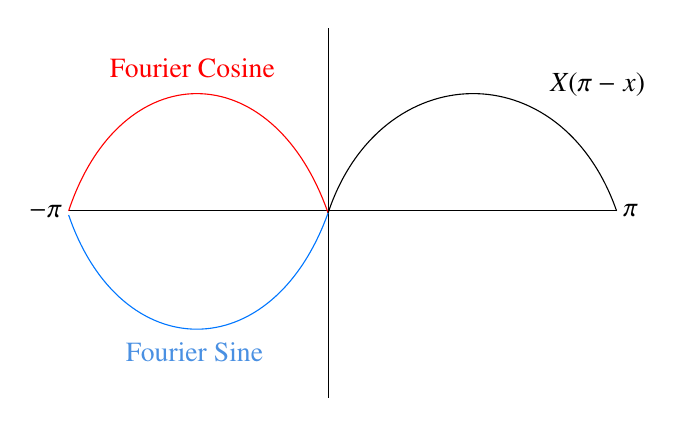
\begin{tikzpicture}[x=0.75pt,y=0.75pt,yscale=-1,xscale=1]
\draw    (104.55,136.99) -- (368.55,136.99) ;
\draw    (229.55,226.99) -- (229.55,48.99) ;
\draw [color={rgb, 255:red, 255; green, 0; blue, 0 }  ,draw opacity=1 ]   (104.55,136.99) .. controls (129.55,61.99) and (202.55,60.99) .. (229.55,137.99) ;
\draw [color={rgb, 255:red, 0; green, 0; blue, 0 }  ,draw opacity=1 ]   (229.55,137.99) .. controls (254.55,62.99) and (341.55,59.99) .. (368.55,136.99) ;
\draw [color={rgb, 255:red, 0; green, 118; blue, 255 }  ,draw opacity=1 ]   (104.55,138.96) .. controls (129.55,212.01) and (202.55,212.98) .. (229.55,137.99) ;
\draw (164.19,73.99) node [anchor=south] [inner sep=0.75pt]  [color={rgb, 255:red, 255; green, 0; blue, 0 }  ,opacity=1 ] [align=left] {Fourier Cosine};
\draw (165.19,199) node [anchor=north] [inner sep=0.75pt]  [color={rgb, 255:red, 74; green, 144; blue, 226 }  ,opacity=1 ] [align=left] {Fourier Sine};
\draw (335,82.98) node [anchor=south west] [inner sep=0.75pt]    {$X( \pi -x)$};
\draw (102.55,136.99) node [anchor=east] [inner sep=0.75pt]    {$-\pi $};
\draw (370.55,136.99) node [anchor=west] [inner sep=0.75pt]    {$\pi $};
\end{tikzpicture}
\end{center}

\section{BVP 2: Vibrating String}

\begin{center}
\tikzset{every picture/.style={line width=0.75pt}}
\begin{tikzpicture}[x=0.75pt,y=0.75pt,yscale=-1,xscale=1]
\draw    (107,180) -- (358,180) ;
\draw [shift={(358,180)}, rotate = 180] [color={rgb, 255:red, 0; green, 0; blue, 0 }  ][line width=0.75]    (0,5.59) -- (0,-5.59)   ;
\draw [shift={(107,180)}, rotate = 180] [color={rgb, 255:red, 0; green, 0; blue, 0 }  ][line width=0.75]    (0,5.59) -- (0,-5.59)   ;
\draw    (107,158) -- (107,70.68) ;
\draw [shift={(107,68.68)}, rotate = 90] [color={rgb, 255:red, 0; green, 0; blue, 0 }  ][line width=0.75]    (10.93,-3.29) .. controls (6.95,-1.4) and (3.31,-0.3) .. (0,0) .. controls (3.31,0.3) and (6.95,1.4) .. (10.93,3.29)   ;
\draw    (107,158) .. controls (113.2,153.35) and (119,141.68) .. (134,141.68) .. controls (149,141.68) and (154.07,163.26) .. (176,166.68) .. controls (197.94,170.09) and (200.47,128.4) .. (217,128.68) .. controls (233.54,128.95) and (218.7,167.85) .. (233,171.68) .. controls (247.31,175.51) and (252.69,133.1) .. (268,131.68) .. controls (283.31,130.26) and (275.18,158.35) .. (286,161.68) .. controls (296.82,165) and (306.53,146.92) .. (323,144.68) .. controls (339.48,142.43) and (354.94,154.98) .. (358,152.68) ;
\draw  [draw opacity=0][fill={rgb, 255:red, 0; green, 0; blue, 0 }  ,fill opacity=1 ] (103.34,161.66) .. controls (103.34,159.64) and (104.98,158) .. (107,158) .. controls (109.02,158) and (110.66,159.64) .. (110.66,161.66) .. controls (110.66,163.68) and (109.02,165.32) .. (107,165.32) .. controls (104.98,165.32) and (103.34,163.68) .. (103.34,161.66) -- cycle ;
\draw  [draw opacity=0][fill={rgb, 255:red, 0; green, 0; blue, 0 }  ,fill opacity=1 ] (350.68,152.68) .. controls (350.68,150.65) and (352.32,149.02) .. (354.34,149.02) .. controls (356.36,149.02) and (358,150.65) .. (358,152.68) .. controls (358,154.7) and (356.36,156.34) .. (354.34,156.34) .. controls (352.32,156.34) and (350.68,154.7) .. (350.68,152.68) -- cycle ;
\draw (105,65.28) node [anchor=south east] [inner sep=0.75pt]    {$\psi $};
\draw (232.5,183.4) node [anchor=north] [inner sep=0.75pt]    {$L$};
\end{tikzpicture}
\end{center}

We now use the Wave Equation 

$\left.a^{2} \dfrac{\partial^{2} \psi}{\partial x^{2}}-\dfrac{\partial^{2} \psi}{\partial t^{2}}=-F\right\} \text { Free vibrations. no external forces. $\therefore\ F=0$}$ 

$\therefore\quad a^{2} \dfrac{\partial^{2} \psi}{\partial x^{2}}=\dfrac{\partial^{2} \psi}{\partial t^{2}}$

We now have the PDE:

$$
\left.\begin{array}{l}
a^{2} \dfrac{\partial^{2} \psi}{\partial x^{2}}=\dfrac{\partial^{2} \psi}{\partial t^{2}} \quad \text { with B.C.s } \\
\psi(0, t)=0,\ \psi(L, t)=0, \text { and I.C.s } \\
\psi(x, 0)=f(x),\ \psi_{t}(x, 0)=g(x)
\end{array}\right\}\text{\textit{Wave Equation with Dirichlet B.C.s}}
$$

Physically, string with fixed/tied ends. Initial displacement of $f(x)$ and initial velocity of $g(x)$. Small vibrations.

Once again, assume $\psi(x, t)=X(x) T(t)$. Plug into PDE:

$$
a^{2} T \dfrac{d^{2} X}{d x^{2}}=X \dfrac{d^{2} T}{d t^{2}}
$$

$\dfrac{1}{X} \dfrac{d^{2} X}{d x^{2}}=\dfrac{1}{a^{2} T} \dfrac{d^{2} T}{d t^{2}}=\lambda$ \textit{This separates to two second-order ODEs}

$$
\dfrac{d^{2} X}{d x^{2}}=\lambda X \quad X(0)=0, X(L)=0
$$

$\left.\begin{array}{l}
     \text{Like in BVP 1A, $\lambda=-\dfrac{n^{2} \pi^{2}}{L^{2}}$ } \\
     X_{n}(x)=A_{n} \sin \left(\dfrac{n \pi x}{L}\right) 
\end{array}\right\}\quad n=1,2, \ldots\text{ because $\sin(0)=0$}.$


$$
\dfrac{d^{2} T}{d t^{2}}=a^{2} \lambda T=-\underbrace{\dfrac{a^{2} n^{2} \pi^{2}}{L^{2}}}_{w_n^2} T,\quad w_{n}=\dfrac{a n \pi}{L}
$$

Allowed angular frequencies of vibration ($n=1,2,3, \ldots$)

$\therefore \dfrac{d^{2} T}{d t^{2}}=-w_{n}^{2} T$ 

General solution is:

$\left.T_{n}(t)=B_{n}^{\prime} \cos \left(w_{n} t\right)+C_{n}^{\prime} \sin \left(w_{n} t\right)\right\}\quad\text { Both $\sin$ and $\cos$ terms exist because $IC \neq B C$, $I C$ is not homogeneous.}$

$$
\psi_{n}(x, t)=\sin \left(\dfrac{n \pi x}{L}\right)\left[B_{n} \cos \left(W_{n} t\right)+C_{n} \sin (W_n t)\right] \begin{aligned}
& B_{n}=B_{n}^{\prime} \cdot A_{n} \\ 
& C_{n}=C'_{n} \cdot A_{n}
\end{aligned}\quad n=1,2, \ldots
$$

Like before, we can rarely satisfy ICs with a single value of $n$. So we use a Fourier Series again

$$
\therefore\underbrace{\left[a^{2} \dfrac{\partial^{2}}{\partial x^{2}}-\dfrac{\partial^{2}}{\partial t^{2}}\right]}_{\mathcal{L}\text{ (a linear operator)}} \psi(x, t)=0\quad \text { find nullspace of } \mathcal{L}.
$$

\[
\boxed{
\psi(x, t) = \sum\limits_{n=1}^{\infty} \sin\left(\dfrac{n \pi x}{L}\right) \left[ B_{n} \cos\left(\omega_{n} t\right) + C_{n} \sin\left(\omega_{n} t\right) \right]
}
\]

Apply position IC for $B_n$:

$\psi(x, 0)=f(x)=\sum\limits_{n=1}^{\infty} B_{n} \sin \left(\dfrac{n \pi x}{L}\right)$ \textit{Using process in BVP 1}:

\[
\boxed{
B_{n} = \dfrac{2}{L} \int\limits_{0}^{L} f{(x)} \sin\left(\dfrac{n \pi x}{L}\right) \, dx
}
\]

Apply velocity IC for $C_{n}$:

\[
\begin{aligned}
\psi_{t}(x, 0) &= \sum\limits_{n=1}^{\infty} C_{n} w_{n} \sin \left( \dfrac{n \pi x}{L} \right) = g(x) \\
\therefore\ & \boxed{ C_{n} w_{n} = \dfrac{2}{L} \int\limits_{0}^{L} g(x) \sin \left( \dfrac{n \pi x}{L} \right) \, dx }
\end{aligned}
\]

Sub in $B_{n}$ and $C_{n}$ for the particular solution.

\section{Newton's Law of Heating and Cooling}

\begin{center}

\tikzset{every picture/.style={line width=0.75pt}}
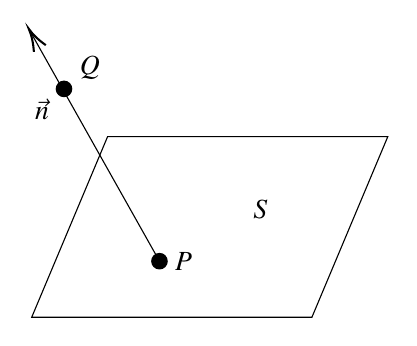
\begin{tikzpicture}[x=0.75pt,y=0.75pt,yscale=-1,xscale=1]
\draw   (136.55,126) -- (271.55,126) -- (235,212.99) -- (100,212.99) -- cycle ;
\draw    (161.55,185.99) -- (99.53,75.73) ;
\draw [shift={(98.55,73.99)}, rotate = 60.64] [color={rgb, 255:red, 0; green, 0; blue, 0 }  ][line width=0.75]    (10.93,-3.29) .. controls (6.95,-1.4) and (3.31,-0.3) .. (0,0) .. controls (3.31,0.3) and (6.95,1.4) .. (10.93,3.29)   ;
\draw  [draw opacity=0][fill={rgb, 255:red, 0; green, 0; blue, 0 }  ,fill opacity=1 ] (157.54,185.99) .. controls (157.54,183.78) and (159.33,181.98) .. (161.55,181.98) .. controls (163.76,181.98) and (165.55,183.78) .. (165.55,185.99) .. controls (165.55,188.2) and (163.76,189.99) .. (161.55,189.99) .. controls (159.33,189.99) and (157.54,188.2) .. (157.54,185.99) -- cycle ;
\draw  [draw opacity=0][fill={rgb, 255:red, 0; green, 0; blue, 0 }  ,fill opacity=1 ] (111.54,102.99) .. controls (111.54,100.78) and (113.33,98.98) .. (115.55,98.98) .. controls (117.76,98.98) and (119.55,100.78) .. (119.55,102.99) .. controls (119.55,105.2) and (117.76,106.99) .. (115.55,106.99) .. controls (113.33,106.99) and (111.54,105.2) .. (111.54,102.99) -- cycle ;
\draw (121.55,99.59) node [anchor=south west] [inner sep=0.75pt]    {$Q$};
\draw (109.54,106.39) node [anchor=north east] [inner sep=0.75pt]    {$\vec{n}$};
\draw (167.55,185.99) node [anchor=west] [inner sep=0.75pt]    {$P$};
\draw (205.55,160.99) node [anchor=west] [inner sep=0.75pt]    {$S$};
\end{tikzpicture}
\end{center}

$\psi_{S}=$ Temperature on surface $S$.

$\psi_{med}=$ Temperature of external medium.

$$
\left[\dfrac{\partial \psi}{\partial n}\right]_{S}=k\left[\psi_{S}-\psi_{me d}\right]
$$

Cooling.

$\psi_{Q}<\psi_{P},\quad \therefore\left[\dfrac{\partial \psi}{\partial n}\right]_{S}<0 \quad \text{Point $Q$ is colder than $P$, causing $S$ to cool down}$.

Therefore, $\left[\dfrac{\partial \psi}{\partial n}\right]_{S}=-k[\parrow{\psi_{S}-\psi_{med}}{$(positive)$, since external medium is colder in cooling}]$

$$
\therefore\left[\dfrac{\partial \psi}{\partial n}+k \psi\right]_{S}=k \psi_{med}
$$


Heating.

$$
\psi_{Q}>\psi_{P}, \quad \therefore\left[\dfrac{\partial \psi}{\partial n}\right]_{S}>0
$$

Therefore, $\left[\dfrac{\partial \psi}{\partial n}\right]_{S}=-k[\parrow{\psi_{S}-\psi_{med}}{$(negative)$, since external medium is hotter in heating}]$

$$
\therefore\left[\dfrac{\partial \psi}{\partial n}+k \psi\right]_{S}=k \psi_{med}
$$

\section{BVP 3: Steady-State Temperature in Rectangular Regions}

Recall Fourier Diffusion Equation:

$$
\dfrac{1}{\alpha^{2}} \dfrac{\partial \psi}{\partial t}-\nabla^{2} \psi=\dfrac{Q}{K} \quad \text { \textit{Steady-state,} } \dfrac{\partial \psi}{\partial t}=0
$$

This reduces to Laplace's Equation if $Q=0$

$$
\therefore \nabla^{2} \psi=0
$$

For $2 D, \dfrac{\partial^{2} \psi}{\partial x^{2}}+\dfrac{\partial^{2} \psi}{\partial y^{2}}=0$

Eg. Rectangular region insulated on 3 sides:

\begin{center}


% Pattern Info
 
\tikzset{
pattern size/.store in=\mcSize, 
pattern size = 5pt,
pattern thickness/.store in=\mcThickness, 
pattern thickness = 0.3pt,
pattern radius/.store in=\mcRadius, 
pattern radius = 1pt}
\makeatletter
\pgfutil@ifundefined{pgf@pattern@name@_rlpbvth38}{
\pgfdeclarepatternformonly[\mcThickness,\mcSize]{_rlpbvth38}
{\pgfqpoint{0pt}{-\mcThickness}}
{\pgfpoint{\mcSize}{\mcSize}}
{\pgfpoint{\mcSize}{\mcSize}}
{
\pgfsetcolor{\tikz@pattern@color}
\pgfsetlinewidth{\mcThickness}
\pgfpathmoveto{\pgfqpoint{0pt}{\mcSize}}
\pgfpathlineto{\pgfpoint{\mcSize+\mcThickness}{-\mcThickness}}
\pgfusepath{stroke}
}}
\makeatother

% Pattern Info
 
\tikzset{
pattern size/.store in=\mcSize, 
pattern size = 5pt,
pattern thickness/.store in=\mcThickness, 
pattern thickness = 0.3pt,
pattern radius/.store in=\mcRadius, 
pattern radius = 1pt}
\makeatletter
\pgfutil@ifundefined{pgf@pattern@name@_nj33ayzxi}{
\pgfdeclarepatternformonly[\mcThickness,\mcSize]{_nj33ayzxi}
{\pgfqpoint{0pt}{-\mcThickness}}
{\pgfpoint{\mcSize}{\mcSize}}
{\pgfpoint{\mcSize}{\mcSize}}
{
\pgfsetcolor{\tikz@pattern@color}
\pgfsetlinewidth{\mcThickness}
\pgfpathmoveto{\pgfqpoint{0pt}{\mcSize}}
\pgfpathlineto{\pgfpoint{\mcSize+\mcThickness}{-\mcThickness}}
\pgfusepath{stroke}
}}
\makeatother

% Pattern Info
 
\tikzset{
pattern size/.store in=\mcSize, 
pattern size = 5pt,
pattern thickness/.store in=\mcThickness, 
pattern thickness = 0.3pt,
pattern radius/.store in=\mcRadius, 
pattern radius = 1pt}
\makeatletter
\pgfutil@ifundefined{pgf@pattern@name@_w9oc5r7rf}{
\pgfdeclarepatternformonly[\mcThickness,\mcSize]{_w9oc5r7rf}
{\pgfqpoint{0pt}{-\mcThickness}}
{\pgfpoint{\mcSize}{\mcSize}}
{\pgfpoint{\mcSize}{\mcSize}}
{
\pgfsetcolor{\tikz@pattern@color}
\pgfsetlinewidth{\mcThickness}
\pgfpathmoveto{\pgfqpoint{0pt}{\mcSize}}
\pgfpathlineto{\pgfpoint{\mcSize+\mcThickness}{-\mcThickness}}
\pgfusepath{stroke}
}}
\makeatother
\tikzset{every picture/.style={line width=0.75pt}} %set default line width to 0.75pt        

\begin{tikzpicture}[x=0.75pt,y=0.75pt,yscale=-1,xscale=1]
%uncomment if require: \path (0,300); %set diagram left start at 0, and has height of 300

%Shape: Square [id:dp22227874357834732] 
\draw   (100,119) -- (194,119) -- (194,213) -- (100,213) -- cycle ;
%Shape: Rectangle [id:dp2410048793786299] 
\draw  [draw opacity=0][pattern=_rlpbvth38,pattern size=6pt,pattern thickness=0.75pt,pattern radius=0pt, pattern color={rgb, 255:red, 0; green, 0; blue, 0}] (79,119) -- (100,119) -- (100,212.68) -- (79,212.68) -- cycle ;
%Shape: Rectangle [id:dp7774032370314381] 
\draw  [draw opacity=0][pattern=_nj33ayzxi,pattern size=6pt,pattern thickness=0.75pt,pattern radius=0pt, pattern color={rgb, 255:red, 0; green, 0; blue, 0}] (100,234) -- (100,213) -- (193.68,213) -- (193.68,234) -- cycle ;
%Shape: Rectangle [id:dp34963124113084665] 
\draw  [draw opacity=0][pattern=_w9oc5r7rf,pattern size=6pt,pattern thickness=0.75pt,pattern radius=0pt, pattern color={rgb, 255:red, 0; green, 0; blue, 0}] (215.01,119) -- (194,119) -- (194,212.71) -- (215.01,212.71) -- cycle ;
%Straight Lines [id:da8816958709447322] 
\draw    (100,115) -- (100,90.68) ;
\draw [shift={(100,88.68)}, rotate = 90] [color={rgb, 255:red, 0; green, 0; blue, 0 }  ][line width=0.75]    (10.93,-4.9) .. controls (6.95,-2.3) and (3.31,-0.67) .. (0,0) .. controls (3.31,0.67) and (6.95,2.3) .. (10.93,4.9)   ;
%Straight Lines [id:da5696131882066631] 
\draw    (133,115) -- (133,90.68) ;
\draw [shift={(133,88.68)}, rotate = 90] [color={rgb, 255:red, 0; green, 0; blue, 0 }  ][line width=0.75]    (10.93,-4.9) .. controls (6.95,-2.3) and (3.31,-0.67) .. (0,0) .. controls (3.31,0.67) and (6.95,2.3) .. (10.93,4.9)   ;
%Straight Lines [id:da8110299108458581] 
\draw    (163,115) -- (163,90.68) ;
\draw [shift={(163,88.68)}, rotate = 90] [color={rgb, 255:red, 0; green, 0; blue, 0 }  ][line width=0.75]    (10.93,-4.9) .. controls (6.95,-2.3) and (3.31,-0.67) .. (0,0) .. controls (3.31,0.67) and (6.95,2.3) .. (10.93,4.9)   ;
%Straight Lines [id:da5340008284668458] 
\draw    (118,113) -- (118,88.68) ;
\draw [shift={(118,115)}, rotate = 270] [color={rgb, 255:red, 0; green, 0; blue, 0 }  ][line width=0.75]    (10.93,-4.9) .. controls (6.95,-2.3) and (3.31,-0.67) .. (0,0) .. controls (3.31,0.67) and (6.95,2.3) .. (10.93,4.9)   ;
%Straight Lines [id:da3811190654784806] 
\draw    (149,114) -- (149,89.68) ;
\draw [shift={(149,116)}, rotate = 270] [color={rgb, 255:red, 0; green, 0; blue, 0 }  ][line width=0.75]    (10.93,-4.9) .. controls (6.95,-2.3) and (3.31,-0.67) .. (0,0) .. controls (3.31,0.67) and (6.95,2.3) .. (10.93,4.9)   ;
%Straight Lines [id:da07417862794483154] 
\draw    (181,114) -- (181,89.68) ;
\draw [shift={(181,116)}, rotate = 270] [color={rgb, 255:red, 0; green, 0; blue, 0 }  ][line width=0.75]    (10.93,-4.9) .. controls (6.95,-2.3) and (3.31,-0.67) .. (0,0) .. controls (3.31,0.67) and (6.95,2.3) .. (10.93,4.9)   ;
%Straight Lines [id:da6344195950034177] 
\draw    (231,119) -- (231,213) ;
\draw [shift={(231,213)}, rotate = 270] [color={rgb, 255:red, 0; green, 0; blue, 0 }  ][line width=0.75]    (0,5.59) -- (0,-5.59)   ;
\draw [shift={(231,119)}, rotate = 270] [color={rgb, 255:red, 0; green, 0; blue, 0 }  ][line width=0.75]    (0,5.59) -- (0,-5.59)   ;
%Straight Lines [id:da046366094265270386] 
\draw    (100,248) -- (193.68,248) ;
\draw [shift={(193.68,248)}, rotate = 180] [color={rgb, 255:red, 0; green, 0; blue, 0 }  ][line width=0.75]    (0,5.59) -- (0,-5.59)   ;
\draw [shift={(100,248)}, rotate = 180] [color={rgb, 255:red, 0; green, 0; blue, 0 }  ][line width=0.75]    (0,5.59) -- (0,-5.59)   ;

% Text Node
\draw (233,166) node [anchor=west] [inner sep=0.75pt]    {$\pi $};
% Text Node
\draw (146.84,251.4) node [anchor=north] [inner sep=0.75pt]    {$\pi $};
% Text Node
\draw (149,78.28) node [anchor=south] [inner sep=0.75pt]    {$T_{0}$};
% Text Node
\draw (98,216.4) node [anchor=north east] [inner sep=0.75pt]    {$0$};


\end{tikzpicture}

\end{center}

Assume $Q=0$

Heats/Cools into a medium at $T_0$

B.C.s $\begin{array}[t]{ll}
     \psi_x(0,y)=0 & \psi_x(\pi,y)=0\\
     \psi_y(x,0)=0 & \left[\dfrac{\partial \psi}{\partial n}+k\psi\right]_{y=\pi}\ =\ \parrow{k}{$(t)$ constant}T_0\text{ (from Newton's law of Heating/Cooling.)}
\end{array}$

This is a well-posed Robin BVP.

Use separation of variables:

$\psi(x, y)=X(x) Y(y)$

$\dfrac{d^{2} X}{d x^{2}} \cdot Y+X \cdot \dfrac{d^{2} Y}{d y^{2}}=0$

\[
\dfrac{1}{X}\dfrac{d^2 X}{dx^2} =- \dfrac{1}{Y}\dfrac{d^2 Y}{dy^2} = \lambda.
\]

$\dfrac{d^{2} X}{d x^{2}}=\lambda X \quad X^{\prime}(0)=0,\quad X^{\prime}(\pi)=0$ This is the same setup in BVP 1B (of which we have the solution of). 

$X_{n}(x)=\left.A_{n} \cos \left(\dfrac{n \pi x}{L}\right)=A_{n} \cos (n x)\right|_{n=\parrow{0}{\text { start at 0 because $\cos (0) \neq 0$}}}\text { with } \lambda=\dfrac{-n^{2} \pi^{2}}{L^{2}}=-\parrow{n^{2}}{In this case, because $L=\pi$}$

$\dfrac{d^{2} Y}{d y^{2}}  =\parrow{-}{The $(-)$ causes $\lambda$ +ve (hyperbolic or exponential)}\lambda Y \quad Y^{\prime}(0)=0 \cdot\left[\dfrac{d^{2}}{d y^{2}}-n^{2}\right] Y=0$

$$
\begin{aligned}
Y_{n}(y) & =B_{n} \cosh (\mu y)+C_{n} \sinh (\mu y) \\
Y_{n}^{\prime}(y) & =-\mu B_{n} \sinh (\mu y)+\mu C_{n} \cosh (\mu y) \quad \text{Applying } Y^{\prime}(0)=0 \\
0 & =-\mu B_{n} \sinh (0)+\mu C_{n} \cosh (0) \qquad \therefore C_{n}=0 \quad(\text {for nonzero } \mu).
\end{aligned}
$$

We can then combine:

\[
\boxed{
\psi_{n}(x, y)=D_{n} \cos \left(\dfrac{n \pi x}{L}\right) \cosh \left(\dfrac{n \pi y}{L}\right)
}
\]

\textit{Important: If the Neumann BCs were Dirichlet instead, simply replace $\cos$ with $\sin$ and $\cosh$ with $\sinh$. The physical interpretation would then become ``3 sides kept at $0^{\circ}$ (or a given constant)''.}

Now we address the case where the 4th B.C. isn't nice (Fourier Series) 

$\therefore Y_{n}(y)=B_{n} \cosh (\mu y) \quad$ Extract $n=0$ term

$$\cosh (0)=1$$
$$
\therefore Y_{0}(y)=B_{0}
$$


\textit{NB: If the bottom edge is the non-constant term, $y$ gets replaced with $\pi-y$ on the hyperbolic.}

Likewise, $\cos (0)=1 \quad \therefore x_{0}(x)=A_{0} \quad \therefore \psi_{0}(x, y)=A_{0} \cdot B_{0}=D_{0}$

$$
\psi(x, y)=\psi_{0}(x, y)+\sum\limits_{n=1}^{\infty} \psi_{n}(x, y)
$$

$\therefore D_{0}+\sum\limits_{n=1}^{\infty} D_{n} \cos (n x) \cosh (n y)$ NB: This is for the case where $L=\pi$. Otherwise keep the argument as $\dfrac{n\pi}{L}$.

Consider 4th BC: $\left[\dfrac{\partial \psi}{\partial n}+k \psi\right]_{y=r}=k T_{0}$

$$\psi_{y}(x, \pi)+k \psi(x, \pi)=k T_{0}$$

$$\sum\limits_{n=1}^{\infty} \parrow{D_{n}}{Pulled out $n=0$ term.} n \sinh (n \pi) \cos (n x)+k {D_{0}}+\sum\limits_{n=1}^{\infty} D_{n} k \cosh (n \pi) \cos (n x)=k T_{0}$$


Collect $D_{n}$ terms:

$\sum\limits_{n=1}^{\infty} D_{n}[n \sinh (n \pi)+k \cosh (n \pi)] \cos (n x)+\overbrace{k D_{0}}^{a_0} \cdot 1=\overbrace{k T_{0}}^{f(x)} \quad$ Fourier Cosine Series

LHS is the Fourier Cosine series of $k T_{0}$

$$
\therefore k D_{0}=\dfrac{1}{\pi} \displaystyle\int\limits_{0}^{\pi} k T_{0} d x=\dfrac{k T_{0} \psi}{\pi}=k T_{0} \Rightarrow D_{0}=T_{0}
$$

$$
D_{n}[n \sinh (n \pi)+k \cosh (n \pi)]=\dfrac{2}{\pi} \displaystyle\int_{0}^{\pi} k T_{0} \cos (n x) d x =\dfrac{2 k T_{0}}{\pi}\left[\dfrac{\sin (n x)}{n}\right]_{0}^{\pi}=0 \quad(\sin (\pi)=0)
$$

Fourier Cosine Series

$$
\begin{aligned}
f(x) & = \dfrac{a_{0}}{2}+\sum\limits_{n=1}^{\infty} a_{n} \cos \left(\dfrac{n \pi x}{L}\right) \\
a_{0} & =\dfrac{2}{L} \displaystyle\int\limits_{0}^{L} f(x) d x \\
a_{n} & =\dfrac{2}{L} \displaystyle\int\limits_{0}^{L} f(x) \cos \left(\dfrac{n \pi x}{L}\right) d x
\end{aligned}
$$

$$
\therefore D_{n}=0,\quad n=1,2, \ldots \quad D_{0}=T_{0} \quad \therefore \psi(x, y)=T_{0}
$$

This makes physical sense. If the only non-insulated side is held at a source at a temperature $T_{0}$, the steady-state temperature of this region will naturally tend towards this $T_{0}$ as time passes. If the non-insulated side has a less predictable heat transfer profile (ie. with spatial dependence, one may simple plug in the given function instead of $kT_{0}$ to the Fourier series and solve for $D_{n}$, before inputting it into the general solution. 

\section{BVP 4: Steady-State Temperature in Circular Regions}

Solve $\nabla^{2} \psi(r, \theta)=0 \quad$ Use Laplacian in polar coordinates.

$$
\nabla^{2} \psi(r, \theta)=\dfrac{1}{r} \dfrac{\partial}{\partial r}\left[r \dfrac{\partial \psi}{\partial r}\right]+\dfrac{1}{r^{2}} \dfrac{\partial^{2} \psi}{\partial \theta^{2}}=0
$$

Let $\psi(r, \theta)=R(r) M(\theta)$

$\dfrac{M}{r} \cdot \dfrac{d}{d r}\left[r \dfrac{d R}{d r}\right]+\dfrac{R}{r^{2}} \cdot \dfrac{d^{2} M}{d \theta^{2}}=0 \quad$ Multiply both sides by $\dfrac{r^{2}}{R M}$

$$
\begin{aligned}
& \dfrac{r}{R} \dfrac{d}{d r}\left[r \dfrac{d R}{d r}\right]+\dfrac{1}{M} \dfrac{d^{2} M}{d \theta^{2}}=0 \\
& \therefore-\dfrac{r}{R} \dfrac{d}{d r}\left[r \dfrac{d R}{d r}\right]=\dfrac{1}{M} \dfrac{d^{2} M}{d \theta^{2}}=\lambda
\end{aligned}
$$

Note that $M$ is periodic with period $2 \pi(M(0)=M(2 \pi))$. Because it is the angular coordinate.

Angular ODE:

$$
\dfrac{d^{2} M}{d \theta^{2}}=\lambda M
$$

Case 1: $\lambda=0\quad \Rightarrow\quad M=A+B \theta$

$B=0$ because $M$ must be periodic.

$$
\therefore M_{0}(\theta)=A_{0}
$$

Case 2: $\lambda$ positive, let $\lambda=\mu^{2}$.

$$
\dfrac{d^{2} M}{d \theta^{2}}=\mu^{2} M,\quad M=\parrow{A \cosh (\mu \theta)}{Not periodic}+\parrow{B \sinh (\mu \theta)}{Not periodic}
$$

$\therefore A=B=0$ (Trivial solution).

Case 3: $\lambda$ negative, let $\lambda=-\mu^{2}$

$\dfrac{d^{2} M}{d \theta^{2}}=-\mu^{2} M, \quad M=A \cos (\mu \theta)+B \sin (\mu \theta). \quad \text { Need } M(2 \pi)=\mu(0).$

$$
\begin{aligned}
& \cos (2 \pi \mu)=\cos (0)  \\
& \sin (2 \pi \mu)=\sin (0)
\end{aligned} \Rightarrow 2 \pi \mu=2 n \pi \quad \therefore \mu=n
$$

Thus; $M_{0}(\theta)=A_{0}. \quad M_{n}(\theta)=A_{n} \cos (n \theta)+B_{n} \sin (n \theta) . \quad n=1,2,3, \ldots$

Radial ODE:

$-\dfrac{r}{d}\left[r \dfrac{d R}{d r}\right]=\lambda=-\parrow{n^{2}}{established that $\mu=n$}$

\[
-\frac{r}{R} \frac{d}{d r}\left[r \frac{d R}{d r}\right]=\lambda=-n^{2}
\]

But only in a full circle. Otherwise, $\lambda=$ ends up being something like $-4 n^{2}$. Go through substitution if not full circle (Roth likes to ask these questions).

Expand the differentials:

$r^{2} \dfrac{d^{2} R}{d r^{2}}+r \dfrac{d R}{d r}-n^{2} R=0$ We solve with the substitution $R=r^{k}$ (Euler ODE).

$$
\begin{array}{ll}
\therefore r^{2} \cdot(k-1) \cdot k \cdot r^{k-2}+r \cdot k \cdot r^{k-1}-n^{2} \cdot r^{k}=0 & \therefore \dfrac{d R}{d r}=k r^{k-1} \\
\left[(k-1) \cdot k+k-n^{2}\right] r^{k}=0\quad \Rightarrow\quad k^{2}-n^{2}=0 \quad \therefore k= \pm n & \therefore \dfrac{d^{2} R}{d r^{2}}=(k-1) k r^{k-2}
 \end{array} 
$$

Thus, $R_{1}=r^{n},\ R_{2}=r^{-n}$

Therefore $R_{n}(r)=C_{n} r^{n}+\dfrac{D_{n}}{r^{n}} \quad n=1,2,3, \ldots$

For $n=0$, we have:

$$
r \dfrac{d}{d r}\left[r \dfrac{d R}{d r}\right]=0 \quad \therefore \dfrac{d}{d r}\Big[\parrow{r \dfrac{d R}{d r}}{Must be constant}\Big]=0 
$$

Integrate both sides:

$\therefore r \dfrac{d R}{d r}=D_{0}$

$\therefore \dfrac{d R}{d r}=\dfrac{D_{0}}{r}\quad \Rightarrow\quad R_{0}(r)=C_{0}+D_{0} \ln (r).$

Now, the final solution to the PDE $\psi(r, \theta)$ is obtained by multiplying $M$ by $R$.

\[
\boxed{
\psi(r, \theta)=E_{0}+F_{0}\ln(r)
+\sum_{n=1}^{\infty}\cos(n\theta)\left[E_{n}r^{n}+\frac{F_{n}}{r^{n}}\right]
+\sum_{n=1}^{\infty}\sin(n\theta)\left[G_{n}r^{n}+\frac{H_{n}}{r^{n}}\right]
}
\]

\textbf{Sectors}

Two sectors possible:

\begin{center}
    

% Pattern Info
 
\tikzset{
pattern size/.store in=\mcSize, 
pattern size = 5pt,
pattern thickness/.store in=\mcThickness, 
pattern thickness = 0.3pt,
pattern radius/.store in=\mcRadius, 
pattern radius = 1pt}
\makeatletter
\pgfutil@ifundefined{pgf@pattern@name@_v13oaedmi}{
\pgfdeclarepatternformonly[\mcThickness,\mcSize]{_v13oaedmi}
{\pgfqpoint{-\mcThickness}{-\mcThickness}}
{\pgfpoint{\mcSize}{\mcSize}}
{\pgfpoint{\mcSize}{\mcSize}}
{
\pgfsetcolor{\tikz@pattern@color}
\pgfsetlinewidth{\mcThickness}
\pgfpathmoveto{\pgfpointorigin}
\pgfpathlineto{\pgfpoint{0}{\mcSize}}
\pgfusepath{stroke}
}}
\makeatother

% Pattern Info
 
\tikzset{
pattern size/.store in=\mcSize, 
pattern size = 5pt,
pattern thickness/.store in=\mcThickness, 
pattern thickness = 0.3pt,
pattern radius/.store in=\mcRadius, 
pattern radius = 1pt}
\makeatletter
\pgfutil@ifundefined{pgf@pattern@name@_7n2nrzda8}{
\pgfdeclarepatternformonly[\mcThickness,\mcSize]{_7n2nrzda8}
{\pgfqpoint{0pt}{0pt}}
{\pgfpoint{\mcSize+\mcThickness}{\mcSize+\mcThickness}}
{\pgfpoint{\mcSize}{\mcSize}}
{
\pgfsetcolor{\tikz@pattern@color}
\pgfsetlinewidth{\mcThickness}
\pgfpathmoveto{\pgfqpoint{0pt}{0pt}}
\pgfpathlineto{\pgfpoint{\mcSize+\mcThickness}{\mcSize+\mcThickness}}
\pgfusepath{stroke}
}}
\makeatother
\tikzset{every picture/.style={line width=0.75pt}} %set default line width to 0.75pt        

\begin{tikzpicture}[x=0.75pt,y=0.75pt,yscale=-1,xscale=1]
%uncomment if require: \path (0,300); %set diagram left start at 0, and has height of 300

%Straight Lines [id:da544818450919442] 
\draw    (71,202) -- (200,202) (81,198) -- (81,206)(91,198) -- (91,206)(101,198) -- (101,206)(111,198) -- (111,206)(121,198) -- (121,206)(131,198) -- (131,206)(141,198) -- (141,206)(151,198) -- (151,206)(161,198) -- (161,206)(171,198) -- (171,206)(181,198) -- (181,206)(191,198) -- (191,206) ;
%Straight Lines [id:da053911973533152135] 
\draw    (71,202) -- (187,148.68) (78.42,194.19) -- (81.76,201.46)(87.5,190.01) -- (90.85,197.28)(96.59,185.84) -- (99.93,193.1)(105.68,181.66) -- (109.02,188.93)(114.76,177.48) -- (118.1,184.75)(123.85,173.31) -- (127.19,180.57)(132.93,169.13) -- (136.28,176.4)(142.02,164.95) -- (145.36,172.22)(151.11,160.78) -- (154.45,168.04)(160.19,156.6) -- (163.53,163.87)(169.28,152.42) -- (172.62,159.69)(178.36,148.25) -- (181.71,155.51) ;
%Curve Lines [id:da7265493688695426] 
\draw    (187,148.68) .. controls (198,163.68) and (201,185.68) .. (200,202) ;
%Straight Lines [id:da11878386180019218] 
\draw    (277,202) -- (406,202) ;
%Straight Lines [id:da984690967716543] 
\draw    (277,202) -- (393,148.68) ;
%Curve Lines [id:da43109495012396026] 
\draw    (393,148.68) .. controls (404,163.68) and (407,185.68) .. (406,202) ;
%Shape: Rectangle [id:dp5279186644390936] 
\draw  [draw opacity=0][pattern=_v13oaedmi,pattern size=6pt,pattern thickness=0.75pt,pattern radius=0pt, pattern color={rgb, 255:red, 0; green, 0; blue, 0}] (277.54,192.77) -- (387.68,141.78) -- (391.14,149.26) -- (281,200.25) -- cycle ;
%Shape: Rectangle [id:dp43271643817006566] 
\draw  [draw opacity=0][pattern=_7n2nrzda8,pattern size=7.5pt,pattern thickness=0.75pt,pattern radius=0pt, pattern color={rgb, 255:red, 0; green, 0; blue, 0}] (277,202) -- (405.5,202) -- (405.5,208.75) -- (277,208.75) -- cycle ;
%Curve Lines [id:da9646808649750684] 
\draw    (304,189.5) .. controls (308.5,190.75) and (309,198.25) .. (306.5,202.25) ;
%Curve Lines [id:da49555289021043625] 
\draw    (101,188.85) .. controls (105.5,190.1) and (106,197.6) .. (103.5,201.6) ;

% Text Node
\draw (135.5,205.4) node [anchor=north] [inner sep=0.75pt]    {$0^{\circ }$};
% Text Node
\draw (127,171.94) node [anchor=south east] [inner sep=0.75pt]    {$0^{\circ }$};
% Text Node
\draw (341.25,208.38) node [anchor=north] [inner sep=0.75pt]   [align=left] {Ins.};
% Text Node
\draw (308.5,198.85) node [anchor=south west] [inner sep=0.75pt]  [font=\footnotesize]  {$\beta $};
% Text Node
\draw (105.5,198.2) node [anchor=south west] [inner sep=0.75pt]  [font=\footnotesize]  {$\beta $};
% Text Node
\draw (202.5,170.2) node [anchor=west] [inner sep=0.75pt]    {$f( \theta )$};
% Text Node
\draw (407.5,171.7) node [anchor=west] [inner sep=0.75pt]    {$f( \theta )$};
% Text Node
\draw (332.34,168.02) node [anchor=south east] [inner sep=0.75pt]   [align=left] {Ins.};
% Text Node
\draw (43,122.5) node [anchor=north west][inner sep=0.75pt]   [align=left] {a)};
% Text Node
\draw (100,232.5) node [anchor=north west][inner sep=0.75pt]   [align=left] {(Dirichlet)};
% Text Node
\draw (306.5,233) node [anchor=north west][inner sep=0.75pt]   [align=left] {(Neumann)};
% Text Node
\draw (262.5,123) node [anchor=north west][inner sep=0.75pt]   [align=left] {b)};


\end{tikzpicture}
\end{center}

For both, we separate regularly:

$$
\dfrac{1}{M} \dfrac{d^{2} M}{d \theta^{2}}=-\dfrac{r}{R} \dfrac{d}{d r}\left[r \dfrac{d R}{d r}\right]=\lambda
$$

For (a), angular ODE is:

$$
\dfrac{d^{2} M}{d \theta^{2}}=\lambda M,\quad 
\begin{aligned}
  M(0)=0,\\[1mm]
  M(\beta)=0,
\end{aligned}
\quad \therefore \quad 
M(\theta)=A_{n} \sin\left(\dfrac{n\pi\theta}{\beta}\right)
\quad \text{(Like BVP 1A)} \quad
\begin{array}{l}
  \text{* Ex 15}\\[2mm]
  \text{PSet 4}
\end{array}
$$

For (b), angular ODE is:

$$
\dfrac{d^{2} M}{d \theta^{2}}=\lambda M,\quad 
\begin{aligned}
  M^{\prime}(0)=0,\\[1mm]
  M^{\prime}(\beta)=0,
\end{aligned}
\quad \therefore \quad 
M(\theta)=A_{n} \cos\left(\dfrac{n\pi\theta}{\beta}\right)
\quad \text{(Like BVP 1B)} \quad
\begin{array}{l}
  \text{* Ex 9}\\[2mm]
  \text{Pset 4}
\end{array}
$$

You then multiply these by the general Radial ODE.

\subsection{BVP 4a: Interior of a Disc (Long cylinder)}

\begin{center}
    

% Pattern Info
 
\tikzset{
pattern size/.store in=\mcSize, 
pattern size = 5pt,
pattern thickness/.store in=\mcThickness, 
pattern thickness = 0.3pt,
pattern radius/.store in=\mcRadius, 
pattern radius = 1pt}
\makeatletter
\pgfutil@ifundefined{pgf@pattern@name@_27uc7uulq}{
\pgfdeclarepatternformonly[\mcThickness,\mcSize]{_27uc7uulq}
{\pgfqpoint{0pt}{0pt}}
{\pgfpoint{\mcSize+\mcThickness}{\mcSize+\mcThickness}}
{\pgfpoint{\mcSize}{\mcSize}}
{
\pgfsetcolor{\tikz@pattern@color}
\pgfsetlinewidth{\mcThickness}
\pgfpathmoveto{\pgfqpoint{0pt}{0pt}}
\pgfpathlineto{\pgfpoint{\mcSize+\mcThickness}{\mcSize+\mcThickness}}
\pgfusepath{stroke}
}}
\makeatother
\tikzset{every picture/.style={line width=0.75pt}} %set default line width to 0.75pt        

\begin{tikzpicture}[x=0.75pt,y=0.75pt,yscale=-1,xscale=1]
%uncomment if require: \path (0,300); %set diagram left start at 0, and has height of 300

%Shape: Circle [id:dp844154481482241] 
\draw  [pattern=_27uc7uulq,pattern size=11.100000000000001pt,pattern thickness=0.75pt,pattern radius=0pt, pattern color={rgb, 255:red, 74; green, 144; blue, 226}] (100,160.5) .. controls (100,130.95) and (123.95,107) .. (153.5,107) .. controls (183.05,107) and (207,130.95) .. (207,160.5) .. controls (207,190.05) and (183.05,214) .. (153.5,214) .. controls (123.95,214) and (100,190.05) .. (100,160.5) -- cycle ;
%Straight Lines [id:da6570586936151104] 
\draw    (58.5,160.5) -- (248.5,160.5) ;
%Straight Lines [id:da12490192807323486] 
\draw    (153.5,79.75) -- (153.5,241.25) ;
%Straight Lines [id:da9230414193174483] 
\draw    (153.5,160.5) -- (189.53,127.35) ;
\draw [shift={(191,126)}, rotate = 137.39] [color={rgb, 255:red, 0; green, 0; blue, 0 }  ][line width=0.75]    (10.93,-4.9) .. controls (6.95,-2.3) and (3.31,-0.67) .. (0,0) .. controls (3.31,0.67) and (6.95,2.3) .. (10.93,4.9)   ;

% Text Node
\draw (170.25,139.85) node [anchor=south east] [inner sep=0.75pt]    {$a$};
% Text Node
\draw (250.5,157.1) node [anchor=south west] [inner sep=0.75pt]    {$f( \theta )$};


\end{tikzpicture}

\end{center}

$$
\begin{array}{ll}
\nabla^{2}(r, \theta)=0 ; & 0 \leqslant r \leqslant a \\
\psi(a, \theta)=f(\theta) & 0 \leqslant \theta \leqslant 2 \pi
\end{array}
$$

We invoke the general solution:

$$
\psi(r, \theta)=E_{0}+F_{0} \ln (r)+\sum\limits_{n=1}^{\infty} \cos (n \theta)\left[E_{n} r^{n}+\dfrac{F_{n}}{r^{n}}\right]+\sum\limits_{n=1}^{\infty} \sin (n \theta)\left[G_{n} r^{n}+\dfrac{H_{n}}{r^{n}}\right]
$$

The solution must be finite for $r=0.\quad \therefore F_{0}=0,\ F_{n}=0,\ H_{n}=0$.

\[
\boxed{
\psi_{\text{INT}}(r, \theta)=E_{0}+\sum_{n=1}^{\infty}E_{n}r^{n}\cos(n\theta)
+\sum_{n=1}^{\infty}G_{n}r^{n}\sin(n\theta)
}
\]

Now we apply the IC to solve for the constants:

$$
\psi_{\text {INT }}(a, \theta)=E_{0}+\sum\limits_{n=1}^{\infty} E_{n} a^{n} \cos (n \theta)+\sum\limits_{n=1}^{\infty} G_{n} a^{n} \sin (n \theta)=f(\theta)
$$

Fourier Series.

$$
\begin{aligned}
& \displaystyle\int_{0}^{2 \pi} \underbrace{E_{0} \cos (k \theta)\, d\theta}_{=0}
+\sum\limits_{n=1}^{\infty} E_{n} a^{n} \displaystyle\int_{0}^{2 \pi} \underbrace{\cos (k \theta) \cos (n \theta)\, d\theta}_{=\pi\cdot \delta_{n,k}}
+\sum\limits_{n=1}^{\infty} G_{n} a^{n} \displaystyle\int_{0}^{2 \pi} \underbrace{\cos (k \theta) \sin (k \theta)\, d\theta}_{=0} \\
& =\displaystyle\int_{0}^{2 \pi} \cos (k \theta) f(\theta)\, d\theta
\end{aligned}
$$

Only nonzero term is when $n=k$. So interchange $k=n$.

$\pi E_{n} a^{n}=\displaystyle\int_{0}^{2 \pi} f(\theta) \cos (n \theta)\, d\theta$

\begin{equation}\tag{1}
\boxed{E_{n}=\dfrac{1}{a^{n} \pi} \displaystyle\int_{0}^{2 \pi} f(\theta) \cos (n \theta)\, d\theta}
\end{equation}

Doing the same thing with $\sin$, we get:

\begin{equation}\tag{2}
\boxed{G_{n}=\dfrac{1}{a^{n} \pi} \displaystyle\int_{0}^{2 \pi} f(\theta) \sin(n \theta)\, d\theta}
\end{equation}

Finally, doing the same thing with 1:

$\displaystyle\int_{0}^{2 \pi} f(\theta) d \theta=\underbrace{E_{0} \displaystyle\int_{0}^{2 \pi} 1 d \theta}_{E_0\cdot 2\pi}+\sum\limits_{n=1}^{\infty} E_{n} a^{n} \displaystyle\int_{0}^{2 \pi} \underbrace{1 \cdot \cos (n \pi)}_{0} d \theta+\sum\limits_{n=1}^{\infty} G_{n} a^{n} \displaystyle\int_{0}^{2 \pi} \underbrace{1 \cdot \sin (n \theta)}_{0} d \theta$

\begin{equation}\tag{3}
\boxed{\therefore E_{0}=\dfrac{1}{2 \pi} \displaystyle\int_{0}^{2 \pi} f(\theta)\, d\theta}
\end{equation}


Plug (1), (2), (3) for $E_{n}, G_{n}, E_{0}$ in the General Solution

\subsection{BVP 4b: Exterior of a Disc (Long cylinder)}

\begin{center}
    

% Pattern Info
 
\tikzset{
pattern size/.store in=\mcSize, 
pattern size = 5pt,
pattern thickness/.store in=\mcThickness, 
pattern thickness = 0.3pt,
pattern radius/.store in=\mcRadius, 
pattern radius = 1pt}
\makeatletter
\pgfutil@ifundefined{pgf@pattern@name@_h2veyrxop}{
\pgfdeclarepatternformonly[\mcThickness,\mcSize]{_h2veyrxop}
{\pgfqpoint{0pt}{0pt}}
{\pgfpoint{\mcSize+\mcThickness}{\mcSize+\mcThickness}}
{\pgfpoint{\mcSize}{\mcSize}}
{
\pgfsetcolor{\tikz@pattern@color}
\pgfsetlinewidth{\mcThickness}
\pgfpathmoveto{\pgfqpoint{0pt}{0pt}}
\pgfpathlineto{\pgfpoint{\mcSize+\mcThickness}{\mcSize+\mcThickness}}
\pgfusepath{stroke}
}}
\makeatother
\tikzset{every picture/.style={line width=0.75pt}} %set default line width to 0.75pt        

\begin{tikzpicture}[x=0.75pt,y=0.75pt,yscale=-1,xscale=1]
%uncomment if require: \path (0,300); %set diagram left start at 0, and has height of 300

%Shape: Rectangle [id:dp22826312156570872] 
\draw  [draw opacity=0][pattern=_h2veyrxop,pattern size=12.899999999999999pt,pattern thickness=0.75pt,pattern radius=0pt, pattern color={rgb, 255:red, 74; green, 144; blue, 226}] (65,86) -- (248,86) -- (248,230) -- (65,230) -- cycle ;
%Shape: Circle [id:dp844154481482241] 
\draw  [fill={rgb, 255:red, 255; green, 255; blue, 255 }  ,fill opacity=1 ] (100,160.5) .. controls (100,130.95) and (123.95,107) .. (153.5,107) .. controls (183.05,107) and (207,130.95) .. (207,160.5) .. controls (207,190.05) and (183.05,214) .. (153.5,214) .. controls (123.95,214) and (100,190.05) .. (100,160.5) -- cycle ;
%Straight Lines [id:da6570586936151104] 
\draw    (58.5,160.5) -- (248.5,160.5) ;
%Straight Lines [id:da12490192807323486] 
\draw    (153.5,79.75) -- (153.5,241.25) ;
%Straight Lines [id:da9230414193174483] 
\draw    (153.5,160.5) -- (189.53,127.35) ;
\draw [shift={(191,126)}, rotate = 137.39] [color={rgb, 255:red, 0; green, 0; blue, 0 }  ][line width=0.75]    (10.93,-4.9) .. controls (6.95,-2.3) and (3.31,-0.67) .. (0,0) .. controls (3.31,0.67) and (6.95,2.3) .. (10.93,4.9)   ;

% Text Node
\draw (170.25,139.85) node [anchor=south east] [inner sep=0.75pt]    {$a$};
% Text Node
\draw (250.5,157.1) node [anchor=south west] [inner sep=0.75pt]    {$f( \theta )$};


\end{tikzpicture}

\end{center}

$$
\begin{aligned}
& \nabla^{2} \psi(r, \theta)=0: \quad r>a \\
& \psi(a, \theta)=f(x).
\end{aligned}
$$

Once again, we invoke the general solution

$$
\psi(r, \theta)=E_{0}+F_{0} \ln (r)+\sum\limits_{n=1}^{\infty} \cos (n \theta)\left[E_{n} r^{n}+\dfrac{F_{n}}{r^{n}}\right]+\sum\limits_{n=1}^{\infty} \sin (n \theta)\left[G_{n} r^{n}+\dfrac{H_{n}}{r^{n}}\right]
$$

This time, since $r>a$, the solution must be finite as $r \rightarrow \infty$

$$
\therefore F_{0}=0,\ E_{n}=0,\ G_{n}=0
$$

\[
\boxed{
\psi_{\text{EXT}}(r, \theta)=E_{0}+\sum_{n=1}^{\infty}\frac{F_{n}}{r^{n}}\cos(n\theta)+\sum_{n=1}^{\infty}\frac{H_{n}}{r^{n}}\sin(n\theta)
}
\]

We apply the same trick as in BVP 4 a to get coefficients:

\[
\boxed{ E_{0} = \frac{1}{2\pi} \int_{0}^{2\pi} f(\theta)\, d\theta }
\]

\[
\boxed{ F_{n} = \frac{a^{n}}{\pi} \int_{0}^{2\pi} f(\theta)\cos(n\theta)\, d\theta }
\]

\[
\boxed{ H_{n} = \frac{a^{n}}{\pi} \int_{0}^{2\pi} f(\theta)\sin(n\theta)\, d\theta }
\]

Plug these into the General Solution

\subsection{BVP 4c: Annular Regions}

\begin{center}
    

% Pattern Info
 
\tikzset{
pattern size/.store in=\mcSize, 
pattern size = 5pt,
pattern thickness/.store in=\mcThickness, 
pattern thickness = 0.3pt,
pattern radius/.store in=\mcRadius, 
pattern radius = 1pt}
\makeatletter
\pgfutil@ifundefined{pgf@pattern@name@_32ngtcpjq}{
\pgfdeclarepatternformonly[\mcThickness,\mcSize]{_32ngtcpjq}
{\pgfqpoint{0pt}{0pt}}
{\pgfpoint{\mcSize+\mcThickness}{\mcSize+\mcThickness}}
{\pgfpoint{\mcSize}{\mcSize}}
{
\pgfsetcolor{\tikz@pattern@color}
\pgfsetlinewidth{\mcThickness}
\pgfpathmoveto{\pgfqpoint{0pt}{0pt}}
\pgfpathlineto{\pgfpoint{\mcSize+\mcThickness}{\mcSize+\mcThickness}}
\pgfusepath{stroke}
}}
\makeatother
\tikzset{every picture/.style={line width=0.75pt}} %set default line width to 0.75pt        

\begin{tikzpicture}[x=0.6pt,y=0.6pt,yscale=-1,xscale=1]
%uncomment if require: \path (0,300); %set diagram left start at 0, and has height of 300

%Shape: Circle [id:dp7991264988405735] 
\draw  [pattern=_32ngtcpjq,pattern size=12.524999999999999pt,pattern thickness=0.75pt,pattern radius=0pt, pattern color={rgb, 255:red, 74; green, 144; blue, 226}][line width=0.75]  (142.27,142.75) .. controls (142.27,93.06) and (182.55,52.78) .. (232.23,52.78) .. controls (281.92,52.78) and (322.2,93.06) .. (322.2,142.75) .. controls (322.2,192.44) and (281.92,232.72) .. (232.23,232.72) .. controls (182.55,232.72) and (142.27,192.44) .. (142.27,142.75) -- cycle ;
%Shape: Ellipse [id:dp4995803253543547] 
\draw  [fill={rgb, 255:red, 255; green, 255; blue, 255 }  ,fill opacity=1 ][line width=0.75]  (174.57,142.75) .. controls (174.57,110.9) and (200.39,85.09) .. (232.23,85.09) .. controls (264.08,85.09) and (289.9,110.9) .. (289.9,142.75) .. controls (289.9,174.6) and (264.08,200.41) .. (232.23,200.41) .. controls (200.39,200.41) and (174.57,174.6) .. (174.57,142.75) -- cycle ;
%Straight Lines [id:da024867792919991194] 
\draw    (100,142.75) -- (364.46,142.75) ;
%Straight Lines [id:da9798445845630093] 
\draw    (232.23,39.5) -- (232.23,246) ;
%Straight Lines [id:da36522671610011104] 
\draw    (232.23,142.75) -- (175.33,78.5) ;
\draw [shift={(174,77)}, rotate = 48.47] [color={rgb, 255:red, 0; green, 0; blue, 0 }  ][line width=0.75]    (10.93,-4.9) .. controls (6.95,-2.3) and (3.31,-0.67) .. (0,0) .. controls (3.31,0.67) and (6.95,2.3) .. (10.93,4.9)   ;
%Straight Lines [id:da9528232868735056] 
\draw    (232.23,142.75) -- (271.51,107.34) ;
\draw [shift={(273,106)}, rotate = 137.97] [color={rgb, 255:red, 0; green, 0; blue, 0 }  ][line width=0.75]    (10.93,-4.9) .. controls (6.95,-2.3) and (3.31,-0.67) .. (0,0) .. controls (3.31,0.67) and (6.95,2.3) .. (10.93,4.9)   ;
%Straight Lines [id:da5910619096813112] 
\draw    (307,91) -- (353,82) ;
%Straight Lines [id:da3884861068326362] 
\draw    (287,162) -- (379,202) ;

% Text Node
\draw (201.12,113.28) node [anchor=north east] [inner sep=0.75pt]    {$\beta $};
% Text Node
\draw (251.62,120.47) node [anchor=south east] [inner sep=0.75pt]    {$\alpha $};
% Text Node
\draw (354,72.4) node [anchor=north west][inner sep=0.75pt]    {$g( \theta )$};
% Text Node
\draw (381,202) node [anchor=west] [inner sep=0.75pt]    {$f( \theta )$};


\end{tikzpicture}

\end{center}

$$
\begin{array}{rll}
\nabla^{2} \psi(r, \theta)=0, & \alpha<r<\beta & \psi(\alpha, \theta)=f(\theta) \\
& 0<\theta<2 \pi & \psi(\beta, \theta)=g(\theta)
\end{array}
$$

Once again, we invoke the general formula.

$$
\psi(r, \theta)=E_{0}+F_{0} \ln (r)+\sum\limits_{n=1}^{\infty} \cos (n \theta)\left[E_{n} r^{n}+\dfrac{F_{n}}{r^{n}}\right]+\sum\limits_{n=1}^{\infty} \sin (n \theta)\left[G_{n} r^{n}+\dfrac{H_{n}}{r^{n}}\right]
$$

We can't kill any terms, though.

However, we can apply the same trick to create a system of equations

$$\psi(\alpha, \theta)=E_{0}+F_{0} \ln (\alpha)+\sum\limits_{n=1}^{\infty} \cos (n \theta)\left[E_{n} \alpha^{n}+\dfrac{F_{n}}{\alpha^{n}}\right]+\sum\limits_{n=1}^{\infty} \sin (\theta)\left[G_{n} \alpha^{n}+\dfrac{H_{n}}{\alpha^{n}}\right]=f(\theta)$$

$
\begin{aligned}
\therefore & E_{0}+F_{0} \ln (\alpha)=\dfrac{1}{2 \pi} \displaystyle\int_{0}^{2 \pi} f(\theta) d \theta \qquad\textcolor{red}{\bullet}\\
\therefore & E_{n} \alpha^{n}+\dfrac{F_{n}}{\alpha^{n}}=\dfrac{1}{\pi} \displaystyle\int_{0}^{2 \pi} f(\theta) \cos (n \theta) d \theta \qquad\textcolor{blue}{\bullet}\\
\therefore & G_{n} \alpha^{n}+\dfrac{F_{n}}{\alpha^{n}}=\dfrac{1}{\pi} \displaystyle\int_{0}^{2 \pi} f(\theta) \sin (n \theta) d \theta\qquad\textcolor{green}{\bullet}
\end{aligned}$

$$\psi(\beta, \theta)=E_{0}+F_{0} \ln (\beta)+\sum\limits_{n=1}^{\infty} \cos (n \theta)\left[E_{n} \beta^{n}+\dfrac{F_{n}}{\beta^{n}}\right]+\sum\limits_{n=1}^{\infty} \sin (\theta)\left[G_{n} \beta^{n}+\dfrac{H_{n}}{\beta^{n}}\right]=g(\theta)$$ 

$\begin{aligned}
\therefore & E_{0}+F_{0} \ln (B)=\dfrac{1}{2 \pi} \displaystyle\int_{0}^{2 \pi} f(\theta) d \theta\qquad\textcolor{red}{\bullet} \\
\therefore & E_{n} B^{n}+\dfrac{F_{n}}{\beta^{n}}=\dfrac{1}{\pi} \displaystyle\int_{0}^{2 \pi} f(\theta) \cos (n \theta) d \theta\qquad\textcolor{blue}{\bullet} \\
\therefore & G_{n} B^{n}+\dfrac{F_{n}}{\beta^{n}}=\dfrac{1}{\pi} \displaystyle\int_{0}^{2 \pi} f(\theta) \sin (n \theta) d \theta\qquad\textcolor{green}{\bullet}
\end{aligned}
$

For every colour \qquad\textcolor{red}{$\bullet$} \qquad\textcolor{blue}{$\bullet$} \qquad\textcolor{green}{$\bullet$}, there are 2 equations and 2 unknowns. Thus all constant terms can be solved for.

\subsection{BVP 4d: Flow Around a Long Circular Cylinder.}

\begin{center}
    

% Pattern Info
 
\tikzset{
pattern size/.store in=\mcSize, 
pattern size = 5pt,
pattern thickness/.store in=\mcThickness, 
pattern thickness = 0.3pt,
pattern radius/.store in=\mcRadius, 
pattern radius = 1pt}
\makeatletter
\pgfutil@ifundefined{pgf@pattern@name@_kq3ypi3xy}{
\pgfdeclarepatternformonly[\mcThickness,\mcSize]{_kq3ypi3xy}
{\pgfqpoint{0pt}{0pt}}
{\pgfpoint{\mcSize}{\mcSize}}
{\pgfpoint{\mcSize}{\mcSize}}
{
\pgfsetcolor{\tikz@pattern@color}
\pgfsetlinewidth{\mcThickness}
\pgfpathmoveto{\pgfqpoint{0pt}{\mcSize}}
\pgfpathlineto{\pgfpoint{\mcSize+\mcThickness}{-\mcThickness}}
\pgfpathmoveto{\pgfqpoint{0pt}{0pt}}
\pgfpathlineto{\pgfpoint{\mcSize+\mcThickness}{\mcSize+\mcThickness}}
\pgfusepath{stroke}
}}
\makeatother
\tikzset{every picture/.style={line width=0.75pt}} %set default line width to 0.75pt        

\begin{tikzpicture}[x=0.75pt,y=0.75pt,yscale=-1,xscale=1]
%uncomment if require: \path (0,300); %set diagram left start at 0, and has height of 300

%Shape: Circle [id:dp844154481482241] 
\draw  [pattern=_kq3ypi3xy,pattern size=9.600000000000001pt,pattern thickness=0.75pt,pattern radius=0pt, pattern color={rgb, 255:red, 74; green, 144; blue, 226}] (100,160.5) .. controls (100,130.95) and (123.95,107) .. (153.5,107) .. controls (183.05,107) and (207,130.95) .. (207,160.5) .. controls (207,190.05) and (183.05,214) .. (153.5,214) .. controls (123.95,214) and (100,190.05) .. (100,160.5) -- cycle ;
%Straight Lines [id:da6570586936151104] 
\draw    (58.5,160.5) -- (246.5,160.5) ;
\draw [shift={(248.5,160.5)}, rotate = 180] [color={rgb, 255:red, 0; green, 0; blue, 0 }  ][line width=0.75]    (10.93,-3.29) .. controls (6.95,-1.4) and (3.31,-0.3) .. (0,0) .. controls (3.31,0.3) and (6.95,1.4) .. (10.93,3.29)   ;
%Straight Lines [id:da12490192807323486] 
\draw    (153.5,81.75) -- (153.5,241.25) ;
\draw [shift={(153.5,79.75)}, rotate = 90] [color={rgb, 255:red, 0; green, 0; blue, 0 }  ][line width=0.75]    (10.93,-3.29) .. controls (6.95,-1.4) and (3.31,-0.3) .. (0,0) .. controls (3.31,0.3) and (6.95,1.4) .. (10.93,3.29)   ;
%Straight Lines [id:da9230414193174483] 
\draw    (153.5,160.5) -- (189.53,127.35) ;
\draw [shift={(191,126)}, rotate = 137.39] [color={rgb, 255:red, 0; green, 0; blue, 0 }  ][line width=0.75]    (10.93,-4.9) .. controls (6.95,-2.3) and (3.31,-0.67) .. (0,0) .. controls (3.31,0.67) and (6.95,2.3) .. (10.93,4.9)   ;
%Straight Lines [id:da5523900846124561] 
\draw    (272,108) -- (306,108) ;
\draw [shift={(308,108)}, rotate = 180] [color={rgb, 255:red, 0; green, 0; blue, 0 }  ][line width=0.75]    (10.93,-3.29) .. controls (6.95,-1.4) and (3.31,-0.3) .. (0,0) .. controls (3.31,0.3) and (6.95,1.4) .. (10.93,3.29)   ;
%Straight Lines [id:da36890622794230365] 
\draw    (272,121) -- (306,121) ;
\draw [shift={(308,121)}, rotate = 180] [color={rgb, 255:red, 0; green, 0; blue, 0 }  ][line width=0.75]    (10.93,-3.29) .. controls (6.95,-1.4) and (3.31,-0.3) .. (0,0) .. controls (3.31,0.3) and (6.95,1.4) .. (10.93,3.29)   ;
%Straight Lines [id:da9676933775167376] 
\draw    (272,134) -- (306,134) ;
\draw [shift={(308,134)}, rotate = 180] [color={rgb, 255:red, 0; green, 0; blue, 0 }  ][line width=0.75]    (10.93,-3.29) .. controls (6.95,-1.4) and (3.31,-0.3) .. (0,0) .. controls (3.31,0.3) and (6.95,1.4) .. (10.93,3.29)   ;
%Straight Lines [id:da8733432384503574] 
\draw    (272,146) -- (306,146) ;
\draw [shift={(308,146)}, rotate = 180] [color={rgb, 255:red, 0; green, 0; blue, 0 }  ][line width=0.75]    (10.93,-3.29) .. controls (6.95,-1.4) and (3.31,-0.3) .. (0,0) .. controls (3.31,0.3) and (6.95,1.4) .. (10.93,3.29)   ;
%Straight Lines [id:da6075991764501645] 
\draw    (272,158) -- (306,158) ;
\draw [shift={(308,158)}, rotate = 180] [color={rgb, 255:red, 0; green, 0; blue, 0 }  ][line width=0.75]    (10.93,-3.29) .. controls (6.95,-1.4) and (3.31,-0.3) .. (0,0) .. controls (3.31,0.3) and (6.95,1.4) .. (10.93,3.29)   ;
%Straight Lines [id:da005869981077274211] 
\draw    (272,171) -- (306,171) ;
\draw [shift={(308,171)}, rotate = 180] [color={rgb, 255:red, 0; green, 0; blue, 0 }  ][line width=0.75]    (10.93,-3.29) .. controls (6.95,-1.4) and (3.31,-0.3) .. (0,0) .. controls (3.31,0.3) and (6.95,1.4) .. (10.93,3.29)   ;
%Straight Lines [id:da4103166996535601] 
\draw    (272,184) -- (306,184) ;
\draw [shift={(308,184)}, rotate = 180] [color={rgb, 255:red, 0; green, 0; blue, 0 }  ][line width=0.75]    (10.93,-3.29) .. controls (6.95,-1.4) and (3.31,-0.3) .. (0,0) .. controls (3.31,0.3) and (6.95,1.4) .. (10.93,3.29)   ;
%Straight Lines [id:da9605484741851416] 
\draw    (272,196) -- (306,196) ;
\draw [shift={(308,196)}, rotate = 180] [color={rgb, 255:red, 0; green, 0; blue, 0 }  ][line width=0.75]    (10.93,-3.29) .. controls (6.95,-1.4) and (3.31,-0.3) .. (0,0) .. controls (3.31,0.3) and (6.95,1.4) .. (10.93,3.29)   ;

% Text Node
\draw (170.25,139.85) node [anchor=south east] [inner sep=0.75pt]    {$a$};
% Text Node
\draw (323,107) node [anchor=west] [inner sep=0.75pt]    {$\vec{v} =v_{0} \hat{\imath} $};
% Text Node
\draw (151.5,76.35) node [anchor=south east] [inner sep=0.75pt]    {$y$};
% Text Node
\draw (250.5,163.9) node [anchor=north west][inner sep=0.75pt]    {$x$};


\end{tikzpicture}

\end{center}

Assume that there is initially uniform glow parallel to the $x$-axis. Then the cylinder is inserted into the flow. The centre of the cylinder is at the origin.

Originally, $\vec{V}=V_{0}\hat{\imath}\quad \Rightarrow\quad \vec{\nabla} \psi=\dfrac{\partial \psi}{\partial x} \hat{\imath}+\dfrac{\partial \psi}{\partial y} \hat{\jmath}$

When the cylinder is inserted:

$\dfrac{\partial \psi}{\partial x} \rightarrow V_{0}$ and $\dfrac{\partial \psi}{\partial y} \rightarrow 0$

$$
\therefore \psi \rightarrow V_{0} x+c=V_{0} \underbrace{r \cos (\theta)}_{x}+c
$$

We invoke the general solution, extracting the $n=1$ term from cos.

$$
\psi(r, \theta)=E_{0}+F_{0} \ln (r)+\cos (\theta)\left[E_{1} r+\dfrac{F_{R}}{r}\right]+\sum\limits_{n=2}^{\infty} \cos (n \theta)\left[E_{n} r^{n}+\dfrac{F_{n}}{r^{n}}\right]+\sum\limits_{n=1}^{\infty} \sin (n \theta)\left[G_{n} r^{n}+\dfrac{H_{n}}{r^{n}}\right]
$$

$$\psi(r, \theta) \longrightarrow C+V_{0} r \cos (\theta) $$

Kill exponential growth terms for stability

$$
\therefore \psi(r, \theta)=E_{0}+V_0r\cos(\theta)+\sum\limits_{n=1}^{\infty} \dfrac{F_{n}}{r^{n}} \cos (n \theta)+\sum\limits_{n=1}^{\infty} \dfrac{H_{n}}{r^{n}} \sin (n \theta)
$$

Since the circumference of the cylinder is a physical boundary, fluid can't enter or leave the surface.

$$\therefore\left[V_{n}\right]_{r=a}=\left[\overrightarrow{\nabla \psi} \cdot \vec{n}\right]_{r=a}=\left[\dfrac{\partial \psi}{\partial r}\right]_{r=a}=0$$

$$
\dfrac{\partial \psi}{\partial r}=V_{0} \cos (\theta)-\sum\limits_{n=1}^{\infty} \dfrac{n F_{n}}{r_{n+1}} \cos (n \theta)-\sum\limits_{n=1}^{\infty} \dfrac{n F_{n}}{r^{n+1}} \sin (n \theta)
$$

Since $\cos (\theta), \cos (2 \theta), \ldots$ and $\sin (\theta), \sin (2 \theta), \ldots$, are orthogonal, they are linearly independent in the complete Fourier Series.

$$
\begin{aligned}
0 & =\left(V_{0}-\dfrac{F_{1}}{a^{2}}\right) \cos (\theta)-\dfrac{2 F_{2}}{a^{3}} \cos (2 \theta)-\ldots- \\
& -\dfrac{H_{1}}{a^{2}} \sin (\theta)-\dfrac{2 H_{2}}{a^{3}} \sin (2 \theta)
\end{aligned}
$$

$H_{n}=0$ (Otherwise the equation can't equal zero).

And, $V_{0}-\dfrac{F_{1}}{a^{2}}=0\quad \Rightarrow\quad F_{1}=V_{0} a^{2}$. All other $F_{n}$ terms must be 0 (For the same reason that $H_{n}=0$).

$\therefore \psi(r, \theta)=E_{0}+V_{0} r \cos (\theta)+\dfrac{V_{0} a^{2}}{r} \cos (\theta)$. $E_{0}$ is arbitrary, can be disregarded

\[
\boxed{
\therefore \psi(r, \theta)=V_{0} \cos (\theta)+\dfrac{V_{0} a^{2}}{r} \cos (\theta)
}
\]

First term: Effect of pre-existing flow

Second term: Effect of cylinder

%%%%%%%%%%%%%%%%%%%%%%%%%%%%%%%%%%%%%%

Thus, $\vec{V}=\overrightarrow{\nabla \psi}=V_{0} \cos (\theta)\left[1-\dfrac{a^{2}}{r^{2}}\right] \hat{\mu}_{r}-V_{0} \sin (\theta)\left[1+\dfrac{a^{2}}{r^{2}}\right] \hat{\mu}_{\theta}$ and $|\vec{v}|_{r=a}=-2 V_{0} \sin (\theta) \hat{\mu}_{\theta}$ (no radial component at the boundary)

\section{BVP 5: Time-Indepedent Non-Homogenous Aspects}

\subsection{BVP 5a. Diffusion of Heat in a Thin Bar, Ends Maintained at $\beta^{\circ}$ and $\gamma^{\circ}$}

Identical to BVP 1a, but ends are at constant $\beta^{\circ}$ and $\gamma^{\circ}$ instead of $0^{\circ}$

\begin{center}
    

\tikzset{every picture/.style={line width=0.75pt}} %set default line width to 0.75pt        

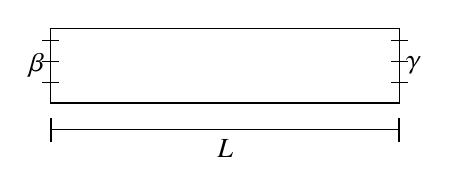
\begin{tikzpicture}[x=0.75pt,y=0.75pt,yscale=-1,xscale=1]
%uncomment if require: \path (0,300); %set diagram left start at 0, and has height of 300

%Shape: Rectangle [id:dp4491854458587017] 
\draw   (141,171) -- (309,171) -- (309,207) -- (141,207) -- cycle ;
%Straight Lines [id:da4657254861857001] 
\draw    (141,207) -- (141,171) (137,197) -- (145,197)(137,187) -- (145,187)(137,177) -- (145,177) ;
%Straight Lines [id:da41979119941170473] 
\draw    (309,207) -- (309,171) (305,197) -- (313,197)(305,187) -- (313,187)(305,177) -- (313,177) ;
%Straight Lines [id:da9943853892815062] 
\draw    (141,220) -- (309,220) ;
\draw [shift={(309,220)}, rotate = 180] [color={rgb, 255:red, 0; green, 0; blue, 0 }  ][line width=0.75]    (0,5.59) -- (0,-5.59)   ;
\draw [shift={(141,220)}, rotate = 180] [color={rgb, 255:red, 0; green, 0; blue, 0 }  ][line width=0.75]    (0,5.59) -- (0,-5.59)   ;

% Text Node
\draw (139,189) node [anchor=east] [inner sep=0.75pt]    {$\beta $};
% Text Node
\draw (311,189) node [anchor=west] [inner sep=0.75pt]    {$\gamma $};
% Text Node
\draw (225,223.4) node [anchor=north] [inner sep=0.75pt]    {$L$};


\end{tikzpicture}

\end{center}

\noindent Diffusion Equation: $\dfrac{1}{\alpha^{2}} \dfrac{\partial \psi}{\partial t}=\dfrac{\partial^{2} \psi}{\partial x^{2}}\, ;\quad 0<x<L,\, t>0$\\[-2ex]

\begin{flushleft}
\begin{tabular}{@{}l@{}}
B.C.s: $\psi(0,t)=\beta,\quad \psi(L,t)=\gamma$\\[1ex]
I.C.: $\psi(x,0)=f(x)$
\end{tabular}
\end{flushleft}

Separation of variables won't work. Instead, we use a Slave Function of one variable to turn the B.C.s homogeneous. The motivation for this is that when subtracted from our initial equation $\psi(x,t)$, the Slave Function $\psi_{S}(x)$ will turn what's left $\psi_{T}(x)$ into a PDE with homogenous B.C.s, which can easily be solved. 

We formalize the "Slave Function" as the "Steady-state" behaviour since it has no time dependency, while $\psi_{T}(x)$ models the transient, or time-dependent, behaviour of the PDE. 

Let $\psi(x, t)=\psi_{S}(x)+\psi_{T}(x, t)$

$\psi_{S}(x)=$ Steady-state temperature.

Sub in this into the PDE:

$\psi_{T}(x, t)=$ Transient temperature.

$$
0+\dfrac{1}{\alpha^{2}} \cdot \dfrac{\partial \psi_{T}}{\partial t}=\dfrac{\partial^{2} \psi_{S}}{\partial x^{2}}+\dfrac{\partial^{2} \psi_{T}}{\partial x^{2}}
$$

First we determine the slave function according to our BC/ICs. 

For the steady-state part, $\dfrac{\partial^{2} \psi_{S}}{\partial x^{2}}=0 \qquad \therefore \psi_{S}(x)=Ax+B$

$$\therefore \psi_{S}(0)=B=\beta\quad \therefore \psi_{S}(x)=A x+\beta$$

$$
\psi_{S}(L)=A L+B=\gamma \quad \therefore A=\dfrac{\gamma-\beta}{L}
$$

Finally, $\boxed{\psi_{S}(x)=\left(\frac{\gamma-\beta}{L}\right)x+\beta}$

In essence, the slave function $\psi_{S}(x)$ "homogenizes" the boundary conditions for the transient function $\psi_{T}(x)$.

For the transient part, $\dfrac{1}{\alpha^{2}} \dfrac{\partial \psi_{T}}{\partial t}=\dfrac{\partial^{2} \psi_{T}}{\partial x^{2}}$

$\left.\begin{array}{l}
    \psi_{T}(0, t)=\psi(0, t)-\psi_{S}(0)=\beta-\beta=0 \quad \text {  Homogeneous. } \\
    \psi_{T}(L, t)=\psi(L, t)-\psi_{S}(L)=\gamma-\gamma=0 \quad \text { Homogeneous. } 
\end{array}\right\}\quad$ B.C.'s

$$
\psi_{T}(x, 0)=\psi(x, 0)-\psi_{S}(x)
=\underbrace{f(x)-\left[\frac{\gamma-\beta}{L}x+\beta\right]}_{F(x)}
\quad \text{I.C.}
$$

The problem is now like BVP 1a. However, keep in mind that the initial condition has changed (from $f(x)$ to $F(x)$ as defined in the line above).

Solve for $\psi_{T}(x, t)$ and add it to $\psi_{S}(x)$ for the final solution. 

Thus, $\psi(x, t)=\psi_{T}(x, t)+\psi_{S}(x)$

$$
\begin{aligned}
& \psi_{T}(x, t)=\dfrac{2}{L} \sum_{n=1}^{\infty} \int_{0}^{L} F(\xi) \sin\left(\dfrac{n \pi \xi}{L}\right)d\xi\, \sin\left(\dfrac{n \pi x}{L}\right)e^{\frac{-\alpha^{2}n^{2}\pi^{2}}{L^{2}}t} \\
& =\int_{0}^{L} G(x, t,\,\xi) F(\xi)d\xi\, ,\quad G(x, t, \xi)=\dfrac{2}{L} \sum_{n=1}^{\infty} \sin\left(\dfrac{n \pi \xi}{L}\right) \sin\left(\dfrac{n \pi x}{L}\right)e^{\frac{-\alpha^{2}n^{2}\pi^{2}}{L^{2}}t}\quad \text{(Green's Function).}
\end{aligned}
$$


\subsection{BVP 5b: Heat Generation/Absorption in a Thin Bar}

This is BVP 1, but with nonzero $Q$.

$$
\dfrac{1}{\alpha^{2}} \cdot \dfrac{\partial \psi}{\partial t}-\nabla^{2} \psi=\dfrac{Q}{K}
$$

Eg.

$$
2 \dfrac{\partial \psi}{\partial t}-\dfrac{\partial^{2} \psi}{\partial x^{2}}=-6 x,\qquad
\begin{aligned}
& \psi(0, t)=3 \quad \psi(x, 0)=x^{3}+2 x+3 \\
& \psi(2, t)=9
\end{aligned}
$$

Let $\psi(x, t)=\psi_{S}(x)+\Phi(x, t) \quad\left(\psi_{T}(x, t)=\Phi(x, t)\right) \quad$ Sub in:

$$
0+2 \dfrac{\partial \Phi}{\partial t}-\dfrac{d^{2} \psi_{S}}{d x^{2}}-\dfrac{\partial^{2} \Phi}{\partial x^{2}}=-6 x
$$

For the slave function $\left(\psi_{S}(x)\right)$, it is in steady state, so $\dfrac{\partial \psi_{S}}{\partial t}=0$

$$\therefore \dfrac{1}{\alpha^{2}}\cdot \dfrac{\partial \psi_{S}}{\partial t}-\nabla^{2} \psi_{S}=\frac{Q}{K} \quad \text { (which is 1 dimensional).}$$

$$-\dfrac{d^{2} \psi_{S}}{d x^{2}}=- 6 x\quad \Rightarrow\quad \psi_{S}(x)=x^{3}+C_{1} x+C_{2} \quad \text { Solve for $C_1,C_2$  using B.C.'s}$$


$$\psi_{S}(0)=C_{2}=3 . \quad \psi_{S}(x)=x^{3}+C_{1} x+3$$

$$\psi_{5}(2)=8+2 C_{1} x+3=9, \quad \therefore C_{1}=-1$$

$$
\therefore \psi_{S}(x)=x^{3}-x+3
$$

Now, address $\Phi(x, t)$ :

$$
\left.\begin{array}{rl}
\text { B.C.'s: } & \Phi(0, t)=\psi(0, t)-\psi_{S}(0)=3-3=0 \\
& \Phi(2, t)=\psi(2, t)-\psi_{S}(2)=9-9=0 \\
\text { I.C: } & \Phi(x, 0)=\left[x^{3}+2 x+3\right]-\left[x^{3}-x+3\right]=3 x
\end{array}\right\} \text{BVP 1a}
$$

$$
\Phi(x, t)=\sum\limits_{n=1}^{\infty} C_{n} \sin \left(\dfrac{n \pi x}{2}\right)e^{\frac{-n^{2} \pi^{2}}{8} t}\quad
$$

$\Phi(x, 0)=\sum\limits_{n=1}^{\infty} C_{n} \sin \left(\dfrac{n \pi x}{2}\right)=3 x \quad$ Fourier Sine Series to resolve IC.

$C_{n}=\dfrac{2}{L}\displaystyle\int_0^L \sin \left(\dfrac{n \pi x}{L}\right) f(x) d x=\dfrac{2}{2} \displaystyle\int_{0}^{2} 3 x \sin \left(\dfrac{n \pi x}{2}\right) d x=\dfrac{-12(-1)^{n}}{n \pi}\quad \text { (Integrate by parts). }$

$$
\therefore \psi(x, t)=\psi_{S}(x)+\Phi(x, t)=x^{3}-x+3-\dfrac{12}{\pi} \sum\limits_{n=1}^{\infty} \dfrac{(-1)^{n}}{n} \sin \left(\dfrac{n \pi x}{2}\right) e^{\frac{-n^{2} \pi^{2}}{8} t}
$$

Physically: $\psi(x, t)$ represents the temperature at a thin rod of length 3, insulated on the sides, initial temperature is $x^{2}+2 x+3$. \quad($Q=$ rate of heat absorption/generation). Diffusivity $\left(\alpha^{2}\right)=\dfrac{1}{2}$. $\dfrac{Q(x)}{k}=-6 x \quad \therefore Q(x)=-6 x k$

\subsection{BVP 5c: Vibrating String with Gravity}

We have $a^{2} \dfrac{\partial^{2} \psi}{\partial x^{2}}-\dfrac{\partial^{2} \psi}{\partial t^{2}}=g$ 

\begin{center}
    

\tikzset{every picture/.style={line width=0.75pt}} %set default line width to 0.75pt        

\begin{tikzpicture}[x=0.75pt,y=0.75pt,yscale=-1,xscale=1]
%uncomment if require: \path (0,300); %set diagram left start at 0, and has height of 300

%Straight Lines [id:da4657254861857001] 
\draw    (141,220) -- (141,196) ;
\draw [shift={(141,196)}, rotate = 90] [color={rgb, 255:red, 0; green, 0; blue, 0 }  ][line width=0.75]    (0,5.59) -- (0,-5.59)   ;
\draw [shift={(141,220)}, rotate = 90] [color={rgb, 255:red, 0; green, 0; blue, 0 }  ][line width=0.75]    (0,5.59) -- (0,-5.59)   ;
%Straight Lines [id:da9943853892815062] 
\draw    (141,220) -- (309,220) ;
%Straight Lines [id:da804925969720879] 
\draw    (309,244) -- (309,220) ;
\draw [shift={(309,220)}, rotate = 90] [color={rgb, 255:red, 0; green, 0; blue, 0 }  ][line width=0.75]    (0,5.59) -- (0,-5.59)   ;
\draw [shift={(309,244)}, rotate = 90] [color={rgb, 255:red, 0; green, 0; blue, 0 }  ][line width=0.75]    (0,5.59) -- (0,-5.59)   ;
%Curve Lines [id:da17066258540314805] 
\draw    (141,196) .. controls (159.2,182.35) and (182.34,206.25) .. (209,222) .. controls (235.66,237.75) and (239,227) .. (249,230) .. controls (259,233) and (276.25,233.83) .. (281,235) .. controls (285.75,236.17) and (301.13,249.9) .. (309,244) ;

% Text Node
\draw (136,208) node [anchor=east] [inner sep=0.75pt]    {$\beta $};
% Text Node
\draw (315,232) node [anchor=west] [inner sep=0.75pt]    {$\gamma $};


\end{tikzpicture}

\end{center}

Ends fixed at $\beta$ and $\gamma$.

B.C.'s: $\psi(0, t)=\beta,\quad \psi(L, t)=\gamma$.

I.C.'s: $\psi(x, 0)=f(x),\quad \psi_{t}(x, 0)=g(x)$.


Use Slave Function

Let $\psi(x, t)=\psi_{S}(x)+\Phi(x, t)$

Substitute into PDE:

$$
a^{2} \dfrac{d^{2} \psi_{S}}{d x^{2}}+\underbrace{a^{2} \dfrac{\partial^{2} \Phi}{\partial x^{2}}- \dfrac{\partial^{2} \Phi}{\partial t^{2}}}_{\text{= 0}}=g
$$

Note that we group our terms such that the transient component is homogeneous. In essence, we split up our inhomogeneous PDE into two: an inhomogeneous ODE $\psi_{S}(x)$ and a homogeneous PDE $\Phi(x,t)$, both of which are solvable. 

$a^{2} \dfrac{d^{2} \psi}{d x^{2}}=g \quad \psi_{S}(0)=\beta, \quad \psi_{S}(L)=\gamma \quad$ Integrate twice

\[
\boxed{
\psi_{S}(x)=-\frac{g x}{2a^{2}}(L-x)+\left(\frac{\gamma-\beta}{L}\right)x+\beta
}
\quad \text{Can be considered the static/equilibrium deflection of the string.}
\]


Once again, we are left with:

$$a^{2} \dfrac{\partial^{2} \Phi}{\partial x^{2}}-\dfrac{\partial^{2} \Phi}{\partial t^{2}}  =0$$

$\left.\begin{array}{ll}
    \text{B.C.'s}: & \Phi(0, t)  =\psi(0, t)-\psi_{S}(0)=\beta-\beta=0 \\
     & \Phi(L, t) =\psi(0, t)-\psi_{S}(0)=\gamma-\gamma=0\\
     \text{I.C.'s}: & \Phi(x, 0)=\psi(x, 0)-\psi_{S}(x)=f(x)-\left\{\dfrac{-g x}{2 a^{2}}(L-x)+\left(\dfrac{\gamma-\beta}{L}\right) x+\beta\right\}=F(x)\\
     & \Phi_{t}(x, 0)=\psi_{t}(x, 0)=g(x)=G(x)
\end{array}\right\}\quad \text{BVP 2}$

As before, sum up $\psi_{S}(x)$ and $\Phi(x,t)$ to obtain $\psi(x,t)$.

\section{BVP 6: Time-Dependent Non-Homogenous Aspects}

\subsection{BVP 6a: Generalized Diffusion, ends at $0^{\circ}$}

General Diffusion Equation: $\dfrac{1}{\alpha^{2}} \dfrac{\partial \psi}{\partial t}-\dfrac{\partial^{2} \psi}{\partial x^{2}}=\parrow{\dfrac{Q(x, t)}{k}}{$\begin{array}{lll}
    \text{In} & \text{BVP 1:} & Q=0 \\
     & \text{BVP 5b:} & Q=f(x)\\
     & \text{BVP 6a:} & Q=f(x,t)
\end{array}$}=h(x, t)$


For simplicity, take $\alpha^{2}=1,\ L=\pi$ (but this can easily be generalized).

Assume ends are maintained at $0^{\circ}$.

$$\therefore \dfrac{\partial \psi}{\partial t}-\dfrac{\partial^{2} \psi}{\partial x^{2}}=h(x, t);\quad 0<x<\pi,\quad t>0$$

\begin{flushleft}
\begin{tabular}{@{}l@{}}
B.C.s: $\psi(0,t)=0,\quad \psi(L,t)=0$\\[1ex]
I.C.: $\psi(x,0)=f(x)$
\end{tabular}
\end{flushleft}


We know the solution for the homogeneous one:

$\psi_{\text {HOM }}(x, t)=\sum\limits_{n=1}^{\infty} C_{n} \sin (n x) e^{-n^{2} t}$ \quad (Complimentary solution).

We can solve with ``Variation of Parameters''.

$$
\text{Let } \boxed{\psi(x, t)=\sum_{n=1}^{\infty} C_{n}(t) \sin (n x)} \text{ *}
$$

(Spatial part satisfies the B.C.'s, so the $e^{-n^{2} t}$ gets incorporated into $C_{n}(t)$.)

Physically, $e^{-n^{2} t}$ represented the decrease with time from an initial temperature of $f(x)$ to O (because there is no heat generation or absorption). However, this term is pointless with nonzero heat generation/absorption.

Sub * into the PDE:

$\sum\limits_{n=1}^{\infty}\left[\dfrac{d C_{n}}{d t}+n^{2} C_{n}\right] \sin (n x)=h(x, t)$ \quad Apply the Fourier Sine trick (all 0 unless $n=k$).

$$
\begin{aligned}
& \sum_{n=1}^{\infty}\left[\frac{d C_{n}}{d t}+n^{2} C_{n}\right] \int_{0}^{\pi} \underbrace{\sin(k x) \sin(n x)\, dx}_{\delta_{k,x}\cdot \frac{\pi}{2}} = \int_{0}^{\pi} \sin(k x) h(x,t)\, dx \\
& \frac{\pi}{2}\left[\frac{d C_{k}}{d t}+k^{2} C_{k}\right]= \int_{0}^{\pi} \sin(k x) h(x,t)\, dx \quad (n=k) \\
& \frac{d C_{n}}{d t}+n^{2} C_{n} = \frac{2}{\pi} \int_{0}^{\pi} \sin(n x) h(x,t)\, dx = B_{n}(t)
\end{aligned}
$$

This is a first-order linear ODE (we solve it by multiplying each side with an integrating factor $\mu(t)$):

$$
\begin{aligned}
& \frac{d C_n}{dt} + \underbrace{n^2 C_n}_{p(t)} = \underbrace{B_n(t)}_{g(t)} \quad \mu(t)= e^{\int p(t)\, dt} = e^{n^2 t} \\
& \underbrace{\frac{d C_n}{dt}\, e^{n^2 t} + n^2 C_n\, e^{n^2 t}}_{\text{reverse prod. rule}} = B_n(t)\, e^{n^2 t}
\end{aligned}
$$


$\dfrac{d}{d t}\left[C_{n} e^{n^{2}t}\right]=B_{n}(t) e^{n^{2} t}$

$\displaystyle\int_{0}^{t} \dfrac{d}{d \tau}\left[C_{n} e^{n^{2} \tau}\right] d \tau=\displaystyle\int_{0}^{t} B_{n}(\tau) e^{n^{2} \tau} d \tau$

$e^{-n^{2}t}\left[C_{n}(t) e^{n^{2} t}-C_{n}(0)\right]=\displaystyle\int_{0}^{t} B_{n}(\tau) e^{n^{2} \tau} d \tau$

$$
\boxed{C_{n}(t)=C_{n}(0) e^{-n^{2} t}+e^{-n^{2} t} \displaystyle\int_{0}^{t} B_{n}(\tau) e^{n^{2} \tau} d \tau}
$$

From the IC: $\psi(x, 0)=\sum\limits_{n=1}^{\infty} C_{n}(0) \sin (n x)=f(x)$

$$
\therefore \boxed{C_{n}(0)=\dfrac{2}{\pi} \displaystyle\int_{0}^{\pi} f(\xi) \sin (n\xi) d\xi}
$$

Plug $C_{n}(t)$ and $C_{n}(0)$ into the (boxed) general solution. $\tau$ and $\xi$ are just dummy variables.

\subsection{BVP 6b. Generalized Diffusion. Dirichlet, B.C. function of time}

\begin{center}
    

\tikzset{every picture/.style={line width=0.75pt}} %set default line width to 0.75pt        

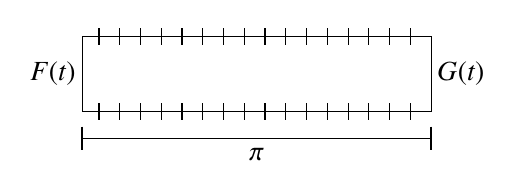
\begin{tikzpicture}[x=0.75pt,y=0.75pt,yscale=-1,xscale=1]
%uncomment if require: \path (0,300); %set diagram left start at 0, and has height of 300

%Shape: Rectangle [id:dp4491854458587017] 
\draw   (141,171) -- (309,171) -- (309,207) -- (141,207) -- cycle ;
%Straight Lines [id:da4657254861857001] 
\draw    (309,171) -- (141,171) (299,175) -- (299,167)(289,175) -- (289,167)(279,175) -- (279,167)(269,175) -- (269,167)(259,175) -- (259,167)(249,175) -- (249,167)(239,175) -- (239,167)(229,175) -- (229,167)(219,175) -- (219,167)(209,175) -- (209,167)(199,175) -- (199,167)(189,175) -- (189,167)(179,175) -- (179,167)(169,175) -- (169,167)(159,175) -- (159,167)(149,175) -- (149,167) ;
%Straight Lines [id:da41979119941170473] 
\draw    (309,207) -- (141,207) (299,211) -- (299,203)(289,211) -- (289,203)(279,211) -- (279,203)(269,211) -- (269,203)(259,211) -- (259,203)(249,211) -- (249,203)(239,211) -- (239,203)(229,211) -- (229,203)(219,211) -- (219,203)(209,211) -- (209,203)(199,211) -- (199,203)(189,211) -- (189,203)(179,211) -- (179,203)(169,211) -- (169,203)(159,211) -- (159,203)(149,211) -- (149,203) ;
%Straight Lines [id:da9943853892815062] 
\draw    (141,220) -- (309,220) ;
\draw [shift={(309,220)}, rotate = 180] [color={rgb, 255:red, 0; green, 0; blue, 0 }  ][line width=0.75]    (0,5.59) -- (0,-5.59)   ;
\draw [shift={(141,220)}, rotate = 180] [color={rgb, 255:red, 0; green, 0; blue, 0 }  ][line width=0.75]    (0,5.59) -- (0,-5.59)   ;

% Text Node
\draw (139,189) node [anchor=east] [inner sep=0.75pt]    {$F( t)$};
% Text Node
\draw (311,189) node [anchor=west] [inner sep=0.75pt]    {$G( t)$};
% Text Node
\draw (225,223.4) node [anchor=north] [inner sep=0.75pt]    {$\pi $};


\end{tikzpicture}

\end{center}

$$\dfrac{\partial\psi}{\partial t}-\dfrac{\partial^2\psi}{\partial t^2}=h(x,t)\qquad \begin{array}{l}
     \psi(0,t)=F(t)  \\
     \psi(\pi,t)=G(t) 
\end{array}\qquad \psi(x,0)=f(t)$$

Now we use a Slave Function of 2 variables. (since the B.C.s are both nonhomogenous and a function of time). Here, the slave function once again represents the long-term behaviour of the system, but this isn't time-indepdent; it just means that the transient components decays relative to the non-constant slave function.

$$\psi(x, t)=\psi_{S}(x, t)+\Phi(x, t)$$

In BVP 5a, we had $\psi(0, t)=\beta,\ \psi(L, t)=\gamma$ with $\psi_{S}(x)=A x+B$.

With the time-variant component, we have:

$$
\psi_{S}(x, t)=A(t) x+B(t)
$$

Thus. $\psi_{S}(0, t)=B(t)$

$\therefore \psi_{S}(x,t)=A(t) x+F(t) \quad$ Now, we incorporate the other B.C.

$\psi_{S}(\pi, t)=A(t) \parrow{\pi}{or generally, $L$}+F(t)=G(t)$

$$
\therefore \boxed{\psi_{S}(x, t)=\left[\dfrac{G(t)-F(t)}{\pi}\right] x+F(t)}
$$

Sub in $\psi(x, t)=\psi_{S}(x, t)+\Phi(x, t)$ into PDE $\dfrac{\partial \psi}{\partial t}-\dfrac{\partial^{2} \psi}{\partial x^{2}}=h(x, t)$.

$$
\therefore\left\{\left[\dfrac{G^{\prime}(t)-F^{\prime}(t)}{\pi}\right] x+F^{\prime}(t)-0\right\}+\dfrac{\partial \Phi}{\partial t}-\dfrac{\partial^{2} \Phi}{\partial x^{2}}+0=h(x, t)
$$

Moving everything to the RHS, we have:

\[
\begin{aligned}
\frac{\partial \Phi}{\partial t} - \frac{\partial^2 \Phi}{\partial x^2} 
&= h(x,t) - \Biggl\{ \left[\frac{G'(t)-F'(t)}{\pi}\right] x + F'(t) \Biggr\}, \\[1ex]
\text{B.C.'s:}\quad \Phi(0,t) 
&= \psi(0,t) - \psi_S(0,t) = F(t) - F(t) = 0, \\[1ex]
\Phi(\pi,t) 
&= \psi(\pi,t) - \psi_S(\pi,t) = G(t) - G(t) = 0, \\[1ex]
\text{I.C.:}\quad \Phi(x,0) 
&= \psi(x,0) - \psi_s(x,0) \\
&= f(x) - \Biggl\{ \left[\frac{G(0)-F(0)}{\pi}\right] x + F(0) \Biggr\} \\
&= \mathcal{F}(x)
\end{aligned}
\]

\begin{flushleft}
As we can see, the PDE of $\Phi(x,t)$ has reduced to an inhomogeneous, time dependent PDE with homogenous B.C.s. This is simply BVP 6a, and we can solve for $\Phi(x,t)$ as we did BVP 6a.

Finally, don't forget to add the slave function to your solution $\psi(x,t)=\Phi(x,t)+\psi_s(x,t)$
\end{flushleft}

\subsection{BVP 6c. Generalized Diffusion. Neumann, B.C. function of time}

\begin{center}
    

\tikzset{every picture/.style={line width=0.75pt}} %set default line width to 0.75pt        

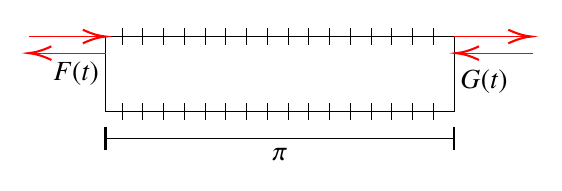
\begin{tikzpicture}[x=0.75pt,y=0.75pt,yscale=-1,xscale=1]
%uncomment if require: \path (0,300); %set diagram left start at 0, and has height of 300

%Shape: Rectangle [id:dp4491854458587017] 
\draw   (141,171) -- (309,171) -- (309,207) -- (141,207) -- cycle ;
%Straight Lines [id:da4657254861857001] 
\draw    (309,171) -- (141,171) (299,175) -- (299,167)(289,175) -- (289,167)(279,175) -- (279,167)(269,175) -- (269,167)(259,175) -- (259,167)(249,175) -- (249,167)(239,175) -- (239,167)(229,175) -- (229,167)(219,175) -- (219,167)(209,175) -- (209,167)(199,175) -- (199,167)(189,175) -- (189,167)(179,175) -- (179,167)(169,175) -- (169,167)(159,175) -- (159,167)(149,175) -- (149,167) ;
%Straight Lines [id:da41979119941170473] 
\draw    (309,207) -- (141,207) (299,211) -- (299,203)(289,211) -- (289,203)(279,211) -- (279,203)(269,211) -- (269,203)(259,211) -- (259,203)(249,211) -- (249,203)(239,211) -- (239,203)(229,211) -- (229,203)(219,211) -- (219,203)(209,211) -- (209,203)(199,211) -- (199,203)(189,211) -- (189,203)(179,211) -- (179,203)(169,211) -- (169,203)(159,211) -- (159,203)(149,211) -- (149,203) ;
%Straight Lines [id:da9943853892815062] 
\draw    (141,220) -- (309,220) ;
\draw [shift={(309,220)}, rotate = 180] [color={rgb, 255:red, 0; green, 0; blue, 0 }  ][line width=0.75]    (0,5.59) -- (0,-5.59)   ;
\draw [shift={(141,220)}, rotate = 180] [color={rgb, 255:red, 0; green, 0; blue, 0 }  ][line width=0.75]    (0,5.59) -- (0,-5.59)   ;
%Straight Lines [id:da8560092446071703] 
\draw [color={rgb, 255:red, 255; green, 0; blue, 0 }  ,draw opacity=1 ]   (104,171) -- (139,171) ;
\draw [shift={(141,171)}, rotate = 180] [color={rgb, 255:red, 255; green, 0; blue, 0 }  ,draw opacity=1 ][line width=0.75]    (10.93,-3.29) .. controls (6.95,-1.4) and (3.31,-0.3) .. (0,0) .. controls (3.31,0.3) and (6.95,1.4) .. (10.93,3.29)   ;
%Straight Lines [id:da2853108945261318] 
\draw [color={rgb, 255:red, 255; green, 0; blue, 0 }  ,draw opacity=1 ]   (106,179) -- (141,179) ;
\draw [shift={(104,179)}, rotate = 0] [color={rgb, 255:red, 255; green, 0; blue, 0 }  ,draw opacity=1 ][line width=0.75]    (10.93,-3.29) .. controls (6.95,-1.4) and (3.31,-0.3) .. (0,0) .. controls (3.31,0.3) and (6.95,1.4) .. (10.93,3.29)   ;
%Straight Lines [id:da5500015788543415] 
\draw [color={rgb, 255:red, 255; green, 0; blue, 0 }  ,draw opacity=1 ]   (309,171) -- (344,171) ;
\draw [shift={(346,171)}, rotate = 180] [color={rgb, 255:red, 255; green, 0; blue, 0 }  ,draw opacity=1 ][line width=0.75]    (10.93,-3.29) .. controls (6.95,-1.4) and (3.31,-0.3) .. (0,0) .. controls (3.31,0.3) and (6.95,1.4) .. (10.93,3.29)   ;
%Straight Lines [id:da9408208078727294] 
\draw [color={rgb, 255:red, 255; green, 0; blue, 0 }  ,draw opacity=1 ]   (312,179) -- (347,179) ;
\draw [shift={(310,179)}, rotate = 0] [color={rgb, 255:red, 255; green, 0; blue, 0 }  ,draw opacity=1 ][line width=0.75]    (10.93,-3.29) .. controls (6.95,-1.4) and (3.31,-0.3) .. (0,0) .. controls (3.31,0.3) and (6.95,1.4) .. (10.93,3.29)   ;

% Text Node
\draw (139,189) node [anchor=east] [inner sep=0.75pt]    {$F( t)$};
% Text Node
\draw (311,193) node [anchor=west] [inner sep=0.75pt]    {$G( t)$};
% Text Node
\draw (225,223.4) node [anchor=north] [inner sep=0.75pt]    {$\pi $};


\end{tikzpicture}

\end{center}

$$\dfrac{\partial \psi}{\partial t}-\dfrac{\partial^2\psi}{\partial x^2}=h(x,t)\qquad \begin{array}{ll}
     \psi_{x}(0, t)=F(t) & \psi(x, 0)=f(t) \\
     \psi_{x}(\pi, t)=G(t) & 
\end{array}$$

Rate of heat inflow (outflow) at ends represented by $F(x), G(x)$.

Same process, assume the general solution is equal to the sum of a transient function and slave function.

$$
\psi(x, t)=\psi_{S}(x, t)+\Phi(x, t)
$$


$\therefore \dfrac{\partial \psi_{S}}{\partial x}=A(t)$. This slave function can't satisfy two derivative-level (Neumann) B.C.s, so we go "up a power".

$\therefore \psi_{S}(x, t)=A(t) x^{2}+B(t) x$

$\therefore \dfrac{\partial \psi_{S}}{\partial x}=2 A(t) x+B(t) \quad \text { Apply B.C.'s: }$

$$
\begin{aligned}
& \left.\dfrac{\partial \psi_{S}}{\partial x}\right|_{x=0}=B(t)=F(t) \\
& \left.\dfrac{\partial \psi_{S}}{\partial x}\right|_{x=\pi}=2 \pi A(t)+F(t)=G(t) \qquad \therefore A(t)=\dfrac{G(t)-F(t)}{2 \pi} 
\end{aligned}
$$

$\therefore \boxed{\psi_{S}(x, t)=\left[\dfrac{G(t)-F(t)}{2 \pi}\right] x^{2}+F(t) x}$

Sub in $\psi(x, t)=\left[\dfrac{G(t)-F(t)}{2 \pi}\right] x^{2}+F(t) x+\Phi(x, t)$ into the PDE:

$$
\begin{aligned}
& \left\{\left[\dfrac{G^{\prime}(t)-F^{\prime}(t)}{2 \pi}\right] x^{2}+F^{\prime}(t) x-\left[\dfrac{G(t)-F(t)}{\pi}\right]\right\}+\dfrac{\partial \Phi}{\partial t}-\dfrac{\partial^{2} \Phi}{\partial x^{2}}=h(x, t) \\
& \dfrac{\partial \Phi}{\partial t}-\dfrac{\partial^{2} \Phi}{\partial x^{2}}=h(x, t)-\left\{\left[\dfrac{G^{\prime}(t)-F^{\prime}(t)}{2 \pi}\right] x^{2}+F^{\prime}(t) x-\left[\dfrac{G(t)-F(t)}{\pi}\right]\right\}=\mathcal{H}(x, t)
\end{aligned}
$$

All that happened was that the RHS of the transient function $\Phi(x,t)$ got modified. In turn, its B.C.s will become homogenous, allowing us to solve for it. We did the same thing in BVP 6b.  

Apply B.C.'s on $\Phi(x, t)$:

$$
\begin{aligned}
& \Phi_{x}(0, t)=\psi_{x}(0, t)-\dfrac{\partial \psi_{S}}{\partial x}(0, t)=F(t)-F(t)=0 \\
& \Phi_{x}(\pi, t)=\psi_{x}(\pi, t)-\dfrac{\partial \psi_{S}}{\partial x}(\pi, t)=G(t)-G(t)=0
\end{aligned}
$$

I.C: $\Phi(x, 0)=\psi(x, 0)-\psi_{S}(x, 0)=f(x)-\left\{\left[\dfrac{G(0)-F(0)}{2 \pi}\right] x^{2}+F(0) x\right\}=\mathcal{F}(x, t)$

Once again. this reduces to BVP 6a. However, with Neumann B.C.s instead of Dirichlet.

With the same reasoning in BVP 6a, we let: 

$$
\Phi(x, t)=\sum\limits_{n=0}^{\infty} C_{n}(t) \cos (n x)=C_{0}(t)+\sum\limits_{n=1}^{\infty} C_{n}(t) \cos (n x)
$$

Sub into PDE:

$\left[\dfrac{d C_{0}}{d t}\right] \cdot 1+\sum\limits_{n=1}^{\infty}\left[\dfrac{d C_{n}}{d t}+n^{2} C_{n}\right] \cos (n x)=\mathcal{H}(x, t) \quad$ Apply Fourier Cosine trick

$$
\begin{aligned}
& \therefore \dfrac{d C_{0}}{d t}=\dfrac{1}{\pi}\int_{0}^{\pi} \mathcal{H}(x,t)\,dx = B_{0}(t) \\
& \therefore \boxed{C_{0}(t)=C_{0}(0)+\int_{0}^{t} B_{0}(\tau)\,d\tau} \\
& \therefore \dfrac{d C_{n}}{d t}+n^{2} C_{n}=\dfrac{2}{\pi}\int_{0}^{\pi} \mathcal{H}(x,t)\cos(nx)\,dx = B_{n}(t)
\end{aligned}
$$

Like in BVP 6a, apply an integrating factor of \(e^{-n^{2}t}\) to get:

$$
\boxed{C_{n}(t)=C_{n}(0)e^{-n^{2}t}+e^{-n^{2}t}\int_{0}^{t} e^{n^{2}\tau} B_{n}(\tau)\,d\tau}
$$

Finally, since
\[
\Phi(x, 0)=C_{0}(0)+\sum_{n=1}^{\infty} C_{n}(0) \cos(nx)=\mathcal{F}(x)
\quad \text{(Fourier Cosine Series)},
\]
we have

$$
\begin{aligned}
& \boxed{C_{0}(0)=\dfrac{1}{\pi}\int_{0}^{\pi} \mathcal{F}(\xi)\,d\xi} \\
& \boxed{C_{n}(0)=\dfrac{2}{\pi}\int_{0}^{\pi} \mathcal{F}(\xi)\cos(n\xi)\,d\xi}
\end{aligned}
$$

Plug and solve for $\Phi(x, t)$. Note that the use of $\tau$ and $\xi$ as variables is just to prevent ambiguity with the $t$ on the bounds of the integrals. Once all computations are done, all these functions are functions of time, $t$.

\section{BVP 7: 3-Variable Diffusion}

Analagous to BVP 3, but not steady state $\left(\dfrac{\partial \psi}{\partial t} \neq 0\right)$

So the temperature is $\psi(x, y, t)$ at any point $P(x, y)$

Assume $\alpha^{2}=1,\ L=\pi$ for simplicity.

\begin{center}
    

\tikzset{every picture/.style={line width=0.75pt}} %set default line width to 0.75pt        

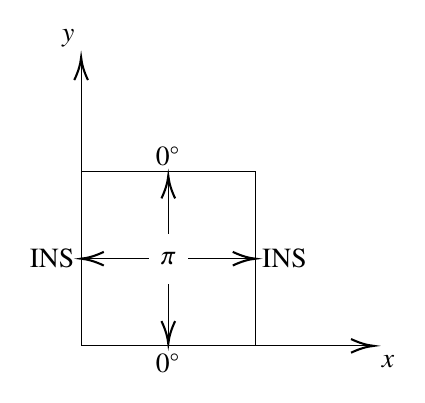
\begin{tikzpicture}[x=0.75pt,y=0.75pt,yscale=-1,xscale=1]
%uncomment if require: \path (0,300); %set diagram left start at 0, and has height of 300

%Shape: Square [id:dp5817550274120495] 
\draw   (100,130) -- (184,130) -- (184,214) -- (100,214) -- cycle ;
%Straight Lines [id:da738039226905576] 
\draw    (100,214) -- (239,214) ;
\draw [shift={(241,214)}, rotate = 180] [color={rgb, 255:red, 0; green, 0; blue, 0 }  ][line width=0.75]    (10.93,-3.29) .. controls (6.95,-1.4) and (3.31,-0.3) .. (0,0) .. controls (3.31,0.3) and (6.95,1.4) .. (10.93,3.29)   ;
%Straight Lines [id:da18159895323009168] 
\draw    (100,214) -- (100,77) ;
\draw [shift={(100,75)}, rotate = 90] [color={rgb, 255:red, 0; green, 0; blue, 0 }  ][line width=0.75]    (10.93,-3.29) .. controls (6.95,-1.4) and (3.31,-0.3) .. (0,0) .. controls (3.31,0.3) and (6.95,1.4) .. (10.93,3.29)   ;
%Straight Lines [id:da5386843576419114] 
\draw    (102,172) -- (182,172) ;
\draw [shift={(184,172)}, rotate = 180] [color={rgb, 255:red, 0; green, 0; blue, 0 }  ][line width=0.75]    (10.93,-3.29) .. controls (6.95,-1.4) and (3.31,-0.3) .. (0,0) .. controls (3.31,0.3) and (6.95,1.4) .. (10.93,3.29)   ;
\draw [shift={(100,172)}, rotate = 0] [color={rgb, 255:red, 0; green, 0; blue, 0 }  ][line width=0.75]    (10.93,-3.29) .. controls (6.95,-1.4) and (3.31,-0.3) .. (0,0) .. controls (3.31,0.3) and (6.95,1.4) .. (10.93,3.29)   ;
%Straight Lines [id:da27606858564834513] 
\draw    (142,211) -- (142,134) ;
\draw [shift={(142,132)}, rotate = 90] [color={rgb, 255:red, 0; green, 0; blue, 0 }  ][line width=0.75]    (10.93,-3.29) .. controls (6.95,-1.4) and (3.31,-0.3) .. (0,0) .. controls (3.31,0.3) and (6.95,1.4) .. (10.93,3.29)   ;
\draw [shift={(142,213)}, rotate = 270] [color={rgb, 255:red, 0; green, 0; blue, 0 }  ][line width=0.75]    (10.93,-3.29) .. controls (6.95,-1.4) and (3.31,-0.3) .. (0,0) .. controls (3.31,0.3) and (6.95,1.4) .. (10.93,3.29)   ;

% Text Node
\draw  [draw opacity=0][fill={rgb, 255:red, 255; green, 255; blue, 255 }  ,fill opacity=1 ]  (132.5,160) -- (151.5,160) -- (151.5,184) -- (132.5,184) -- cycle  ;
\draw (142,172) node    {$\pi $};
% Text Node
\draw (98,71.6) node [anchor=south east] [inner sep=0.75pt]    {$y$};
% Text Node
\draw (243,217.4) node [anchor=north west][inner sep=0.75pt]    {$x$};
% Text Node
\draw (186,172) node [anchor=west] [inner sep=0.75pt]   [align=left] {INS};
% Text Node
\draw (98,172) node [anchor=east] [inner sep=0.75pt]   [align=left] {INS};
% Text Node
\draw (142,128.6) node [anchor=south] [inner sep=0.75pt]    {$0^{\circ }$};
% Text Node
\draw (142,216.4) node [anchor=north] [inner sep=0.75pt]    {$0^{\circ }$};


\end{tikzpicture}

\end{center}

$$
\dfrac{\partial \psi}{\partial t}=\dfrac{\partial^{2} \psi}{\partial x^{2}}+\dfrac{\partial^{2} \psi}{\partial y^{2}}\quad 
\begin{array}[c]{l}
     0<x<\pi \\
     0<y<\pi 
\end{array}\quad 
\underbrace{
\begin{array}[c]{l}
     \psi_x(0,y,t)=0\\
     \psi(\pi,y,t)=0 
\end{array}
}_{\text{2 x Neumann}}\quad 
\underbrace{
\begin{array}[c]{l}
     \psi(x,0,t)=0\\
     \psi(x,\pi,t)=0 
\end{array}
}_{\text{2 x Dirichlet}}\quad \psi(x,y,0)=f(x,y)
$$


Separation of Variables:

$$
\begin{aligned}
& \psi(x, y, t)=X(x) Y(y) T(t)=0 \\
& \begin{array}{ll}
    X^{\prime}(0)=0 & Y(0)=0 \\
    X^{\prime}(\pi)=0 & Y(\pi)=0 
\end{array}
\end{aligned}
$$

$\left\{X Y \dfrac{d T}{d t}=\dfrac{d^{2} X}{d x^{2}} Y T+X \dfrac{d^{2} Y}{d y^{2}} T\right\} \cdot \dfrac{1}{X Y T}$

$\dfrac{1}{T} \dfrac{d T}{d t}=\dfrac{1}{X} \dfrac{d^{2} X}{d x^{2}}+\dfrac{1}{Y} \dfrac{d^{2} Y}{d y^{2}}$

$\dfrac{1}{T} \dfrac{d T}{d t}-\dfrac{1}{Y} \dfrac{d^{2} Y}{d y^{2}}=\dfrac{1}{X} \dfrac{d^{2} X}{d x^{2}}=\text { constant. }=\lambda$

$\dfrac{1}{X} \dfrac{d^{2} X}{d x^{2}}=\lambda,\quad X^{\prime}(0)=0,\ X^{\prime}(\pi)=0\quad \text{BVP 1b}$

$$
\therefore X(x)=A_{n} \cos \left(\frac{n \pi x}{\pi}\right)
=A_{n} \cos (n x),\quad n=0,1,\ldots \qquad \lambda=\frac{n^{2}\pi^{2}}{\pi^{2}}=n^{2}
$$

Now we are left with:

$\dfrac{1}{T} \cdot \dfrac{d T}{d t}-\dfrac{1}{Y} \dfrac{d^{2} Y}{d y^{2}}=\lambda=-n^{2}$

$$\therefore \dfrac{1}{T} \cdot \dfrac{d T}{d t}+n^{2}=\dfrac{1}{Y} \dfrac{d^{2} Y}{d y^{2}}=\text { constant }=\parrow{\mu}{Different from $\lambda$}$$

$\dfrac{d^{2} Y}{d y^{2}}=Y \mu, Y(0)=0, Y(\pi)=0 \quad$ \text{BVP 1a}

$Y(y)=B_{k} \sin (k y), k=1,2,3 \ldots \quad \mu=\parrow{\dfrac{k^{2} \pi^{2}}{\pi^{2}}}{``H''}=k^{\prime 2}$

Finally, $\dfrac{d T}{d t}=T\left(-n^{2}-\mu\right)$

$$
\therefore T(t)=C_{n k} e^{-\left(n^{2}+k^{2}\right) t}
$$

So the complete solution is:

$$
\boxed{\psi_{n k}(x, y, t)=D_{n k} \cos (n x) \sin (k y) e^{-\left(n^{2}+k^{2}\right) t}}
$$

$\cos$ because $x$ B.C.'s are Neumann\\
$\sin$ because $y$ B.C.'s are Dirichlet.

Same Fourier thing as BVP 1, but multivariable:

$$
\left[\dfrac{\partial}{\partial t}-\dfrac{\partial^{2}}{\partial x^{2}}-\dfrac{\partial^{2}}{\partial y^{2}}\right] \psi(x, y, t)=0
$$

$\mathcal{L} \psi=0$. Want nullspace of this linear operator ($\mathcal{L}$ is a linear operator, so we can use superposition)

$$
\therefore \psi(x, y, t)=\sum\limits_{k=1}^{\infty} \sum\limits_{n=0}^{\infty} D_{n k} \cos (n x) \sin (k y) e^{-\left(n^{2}+k^{2}\right) t}
$$

Apply IC, extract $n=0$ term:

$$
\psi(x, y, 0)=\sum\limits_{k=1}^{\infty} D_{0 k} \sin (k y)+\sum\limits_{k=1}^{\infty} \sum\limits_{n=1}^{\infty} D_{n k} \cos (n x) \sin (k y)=f(x, y)
$$

We do the Fourier Sine Trick: (multiply by $\sin(ly)$, take double integral).

$$
\begin{aligned}
& \sum_{k=1}^{\infty} D_{0k} \int_{0}^{\pi} \underbrace{(1)\,dx}_{\pi} \int_{0}^{\pi} \underbrace{\sin(l y)\sin(ky)}_{\delta_{l,k}\cdot \frac{\pi}{2}}\,dy 
+ \sum_{k=1}^{\infty} \sum_{n=1}^{\infty} D_{nk} \int_{0}^{\pi} \underbrace{(1)\cos(nx)\,dx}_{0} \int_{0}^{\pi} \underbrace{\sin(l y)\sin(ky)\,dy}_{\delta_{l,k}\cdot \frac{\pi}{2}}\\[1ex]
&\quad = \int_{0}^{\pi} \int_{0}^{\pi} \sin(l y)f(x,y)\,dx\,dy\quad\text{only nonzero when } l=k,\\[1ex]
& \frac{\pi^2}{2}\, D_{0l} = \int_{0}^{\pi} \int_{0}^{\pi} \sin(l y)f(x,y)\,dx\,dy.
\end{aligned}
$$

$$
\therefore \boxed{D_{0k}=\frac{2}{\pi^{2}} \int_{0}^{\pi} \int_{0}^{\pi} \sin(l y)f(x,y)\,dx\,dy}
$$

Repeat with \(\cos(mx)\sin(ly)\) for \(D_{nk}\) and sub in \(D_{0k}\) and \(D_{nk}\) into the general solution.

$$
\begin{aligned}
& \sum_{k=1}^{\infty} D_{0k} \int_{0}^{\pi} \sin(l y)\sin(ky)\,dy \int_{0}^{\pi} \underbrace{(1)\cos(mx)\,dx}_{0}
+ \sum_{k=1}^{\infty} \sum_{n=1}^{\infty} D_{nk} \int_{0}^{\pi} \underbrace{\cos(mx)\cos(nx)\,dx}_{\frac{\pi}{2}\,\delta_{m,n}} \int_{0}^{\pi} \underbrace{\sin(l y)\sin(ky)\,dy}_{\frac{\pi}{2}\,\delta_{l,k}}\\[1ex]
&\quad = \int_{0}^{\pi} \int_{0}^{\pi} \cos(mx)\sin(ly)f(x,y)\,dx\,dy.
\end{aligned}
$$

$$
\therefore \boxed{D_{nk}=\frac{4}{\pi^{2}} \int_{0}^{\pi} \int_{0}^{\pi} \cos(nx)\sin(ky)f(x,y)\,dx\,dy}
$$

\section{BVP 8: Poisson's Equation}

$$
\nabla^{2} \psi=-F \quad(\text { Poisson's Equation) }
$$

$F$ can represent:

$\psi=$ Velocity Potential, $F=$ Rate of Fluid Generation.\\
$\psi=$ Steady State Temperature, $F=$ Rate of Heat Generation.\\
$\psi=$ Displacement, $F=$ External Force/ mass.\\
$\psi=$ Electric Potential, $F=$ Charge Density.\\
Eg. Steady-State Temp Distribution:

\begin{center}
    

\tikzset{every picture/.style={line width=0.75pt}} %set default line width to 0.75pt        

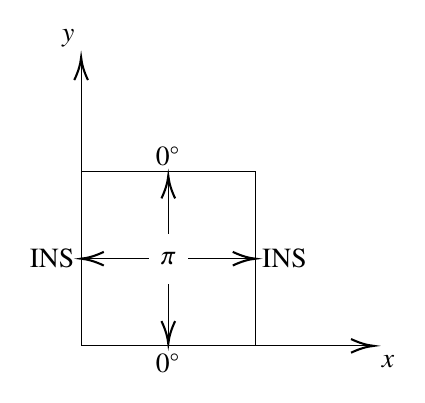
\begin{tikzpicture}[x=0.75pt,y=0.75pt,yscale=-1,xscale=1]
%uncomment if require: \path (0,300); %set diagram left start at 0, and has height of 300

%Shape: Square [id:dp5817550274120495] 
\draw   (100,130) -- (184,130) -- (184,214) -- (100,214) -- cycle ;
%Straight Lines [id:da738039226905576] 
\draw    (100,214) -- (239,214) ;
\draw [shift={(241,214)}, rotate = 180] [color={rgb, 255:red, 0; green, 0; blue, 0 }  ][line width=0.75]    (10.93,-3.29) .. controls (6.95,-1.4) and (3.31,-0.3) .. (0,0) .. controls (3.31,0.3) and (6.95,1.4) .. (10.93,3.29)   ;
%Straight Lines [id:da18159895323009168] 
\draw    (100,214) -- (100,77) ;
\draw [shift={(100,75)}, rotate = 90] [color={rgb, 255:red, 0; green, 0; blue, 0 }  ][line width=0.75]    (10.93,-3.29) .. controls (6.95,-1.4) and (3.31,-0.3) .. (0,0) .. controls (3.31,0.3) and (6.95,1.4) .. (10.93,3.29)   ;
%Straight Lines [id:da5386843576419114] 
\draw    (102,172) -- (182,172) ;
\draw [shift={(184,172)}, rotate = 180] [color={rgb, 255:red, 0; green, 0; blue, 0 }  ][line width=0.75]    (10.93,-3.29) .. controls (6.95,-1.4) and (3.31,-0.3) .. (0,0) .. controls (3.31,0.3) and (6.95,1.4) .. (10.93,3.29)   ;
\draw [shift={(100,172)}, rotate = 0] [color={rgb, 255:red, 0; green, 0; blue, 0 }  ][line width=0.75]    (10.93,-3.29) .. controls (6.95,-1.4) and (3.31,-0.3) .. (0,0) .. controls (3.31,0.3) and (6.95,1.4) .. (10.93,3.29)   ;
%Straight Lines [id:da27606858564834513] 
\draw    (142,211) -- (142,134) ;
\draw [shift={(142,132)}, rotate = 90] [color={rgb, 255:red, 0; green, 0; blue, 0 }  ][line width=0.75]    (10.93,-3.29) .. controls (6.95,-1.4) and (3.31,-0.3) .. (0,0) .. controls (3.31,0.3) and (6.95,1.4) .. (10.93,3.29)   ;
\draw [shift={(142,213)}, rotate = 270] [color={rgb, 255:red, 0; green, 0; blue, 0 }  ][line width=0.75]    (10.93,-3.29) .. controls (6.95,-1.4) and (3.31,-0.3) .. (0,0) .. controls (3.31,0.3) and (6.95,1.4) .. (10.93,3.29)   ;

% Text Node
\draw  [draw opacity=0][fill={rgb, 255:red, 255; green, 255; blue, 255 }  ,fill opacity=1 ]  (132.5,160) -- (151.5,160) -- (151.5,184) -- (132.5,184) -- cycle  ;
\draw (142,172) node    {$\pi $};
% Text Node
\draw (98,71.6) node [anchor=south east] [inner sep=0.75pt]    {$y$};
% Text Node
\draw (243,217.4) node [anchor=north west][inner sep=0.75pt]    {$x$};
% Text Node
\draw (186,172) node [anchor=west] [inner sep=0.75pt]   [align=left] {INS};
% Text Node
\draw (98,172) node [anchor=east] [inner sep=0.75pt]   [align=left] {INS};
% Text Node
\draw (142,128.6) node [anchor=south] [inner sep=0.75pt]    {$0^{\circ }$};
% Text Node
\draw (142,216.4) node [anchor=north] [inner sep=0.75pt]    {$0^{\circ }$};


\end{tikzpicture}

\end{center}

$$\parrow{\nabla^2\psi=-F(x,y)}{$\substack{\text{Unlike BVP 7, PDE is not}\\
\text{homogeneous, but $\frac{\partial\psi}{\partial t}=0$}}$}\qquad \underbrace{\begin{array}[t]{l}
     \psi_x(0,y,t)=0 \\
     \psi_x(\pi,y,t)=0
\end{array}}_{\text{2 x Neumann}} \qquad \underbrace{\begin{array}[t]{l}
     \psi(x,0,t)=0 \\
     \psi(x,\pi,t)=0
\end{array}}_{\text{2 x Dirichlet}}$$

Using the same principle from BVP 7:


\[
\boxed{
\psi(x, y)=\sum_{k=1}^{\infty} \sum_{n=0}^{\infty} C_{nk}\,
\underbrace{\cos (n x)}_{\text{Newman}}\, \underbrace{\sin (k y)}_{\text{Dirichlet}}
}
\]

This satisfies all 4 B.C.'s. Just need the PDE now.

$\nabla^{2} \psi(x, y)=-F(x, y)$. Plug $\psi(x, y)$ into PDE.


\begin{align*}
& \therefore \nabla^{2} \psi(x, y)=\sum\limits_{k=1}^{\infty} \sum\limits_{n=0}^{\infty} C_{n k}\left[-n^{2}-k^{2}\right] \cos (n x) \sin (k y)=-F(x, y) \\
& \therefore \sum\limits_{k=1}^{\infty} \sum\limits_{n=0}^{\infty} C_{n k}\left[n^{2}+k^{2}\right] \cos (n x) \sin (k y)=F(x, y) \tag{1}
\end{align*}


Like in BVP 7, extract the $n=0$ term.

\begin{equation}\tag{2}
    \sum_{k=1}^{\infty} D_{0 k} \sin (k y)+\sum\limits_{k=1}^{\infty} \sum\limits_{n=1}^{\infty} D_{n k} \cos (n x) \sin (k y)=f(x, y) \quad \text { (From BVP 7) }
\end{equation}

Equating (1) and (2) (since we know the solution to (1))

$$
C_{0k} \cdot k^{2} = D_{0k}=\dfrac{2}{\pi^{2}} \int_{0}^{\pi} \int_{0}^{\pi} \sin(ky)\,dx\,dy
$$

$$
C_{nk}\left[n^{2}+k^{2}\right] = D_{nk}=\dfrac{4}{\pi^{2}} \int_{0}^{\pi} \int_{0}^{\pi} \cos(nx)\sin(ky)\,dx\,dy
$$

$$
\boxed{C_{0k}=\dfrac{2}{\pi^{2}k^{2}} \int_{0}^{\pi}\int_{0}^{\pi}\sin(ky)F(x,y)\,dx\,dy}\\[1ex]
$$

$$
\boxed{C_{nk}=\dfrac{4}{\pi^{2}\left(n^{2}+k^{2}\right)} \int_{0}^{\pi}\int_{0}^{\pi}\cos(nx)\sin(ky)F(x,y)\,dx\,dy}
$$


Sub into general solution.

What if B.C.'s are not homogeneous?

Let
\[
\psi(x,y)=\overset{\scriptsize \text{Nonhomogeneous B.C. / Homogeneous PDE. (BVP 3)}}{\psi_H(x,y)}
+\overset{\scriptsize \text{Homogeneous B.C. / Nonhomogeneous PDE. (what we just got)}}{\psi_P(x,y)}.
\]

$$
\nabla^{2} \psi(x, y)=-F(x, y)
$$

We solve the two cases separately and then sum up the results. Note that if multiple B.C.s are not homogenous, they have to be addressed separately. That is, when getting $\psi_{H}(x,y)$, we sequentially consider all but one B.C. to be homogenous and solve, before adding up all results.

See question 4 on page 273 of the coursepack for an example. That being said, this is a pretty tough question and it is hard to think of this on the spot without knowing what to do \emph{a priori}.

\end{document}
